\chapter{Experimental field tests}\label{Ch:ExperimentalTesting}
\section{Outline of testing}
The experimental field tests was performed at Agdenes airfield over the course of two subsequent days with a virtual net placed $26 m$ above the runway, by placing the mobile sensor unit on the runway acting as a reference position in Neptus. The runway at Agdenes has the direction West-East. This is in the experimental testing defining the two possible directions from which the \gls{uav} can perform autonomous landing. The autonomous landing system is applied with the same control system used in the \gls{sil} simulation in section \ref{ss:SILOutline}, with the configuration parameters listen in tables \ref{AP:TB:LOSnSMCuser}, \ref{AP:TB:Longitudianl} and \ref{AP:TB:HeightGlideslope}. It should be noted that the low level controllers in the hardware configuration of the X8 has not been fined tuned for autonomous flight, expected to decrease the performance of the high level controllers compared to the \gls{sil} simulation. Similar to the \gls{sil} simulation the time of arrival factor is set to $2 s$ during the landing plan. The \gls{uav} navigation system used in the autonomous landing operation is the system presented in section \ref{IMP:NavSys}. The \gls{uav} operation is an \gls{los} operation, i.e. the \gls{uav} must be within the line of sight of the pilot at all time.

The weather condition differed over the course of the two days, where the first had windspeeds between $8-9 m/s$ from the West while the second day was considered calm. Hence the performance of the autonomous landing system was tested under two different wind condition, where one strained the performance of the system while the other could be considered as ideal conditions. All landing plan was generated when the \gls{uav} was in a loiter manoeuvre, i.e. in a constant circle manoeuvre around a fixed position. This in order to be able to review the landing plan and confirm that the correct controllers had been assigned before executing the landing plan.
\section{Execution of testing - Day 1 (Windy conditions)}
\subsection{Performed tests}
A total number of 11 test flights were conducted the first day of testing. During these tests three different configuration were tested, in addition to the initial test configuration which was used to determine a baseline for the experimental testing. The initial configuration was determined based on both input from the operator, and early \gls{sil} tests of the system. Further to the initial test configuration, tests with reduced approach angle, inverted turning direction for the start circle and reduced lookahead distance in the lateral control system was carried out.

Table \ref{tb:Day1ParameterAlteration} list up the number of flight test which was perform during the first day, in addition to the state of the autonomous landing system parameter which was altered in one of the three different configuration set-ups. Test number $1-2$ were tests performed with the initial set-up, test number $3$ was a test with reduced final approach angle, test number $4-9$ were tests inverted turning direction for the start circle and test number $10-11$ were tests reduced lookahead distance in the lateral control system.  Only test configuration number $1,3,4$ and $10$ are presented in plots, while all test data are used to determine the overall performance of the autonomous landing system during the first day.
\newpage
\begin{table}[H]
\begin{tabular}{| p{0.5cm} | p{3cm} | p{4cm} | p{4cm} |}
\hline
\textbf{Test Nr.} & \textbf{Final approach angle [deg]} & \textbf{Lateral control system - Lookahead distance [m]} &  \textbf{Rotation combination - approach path}\\ \hline
$1$				& $3$ &	$ 50 $ 	& Clockwise/Counter-clockwise		\\ \hline
$2$				& $3$ & $ 50 $	& Clockwise/Counter-clockwise			\\ \hline
$3$				& $0$ & $ 50 $	& Clockwise/Counter-clockwise		\\ \hline
$4$				& $0$ & $ 50 $ 	& Counter-clockwise/ Counter-clockwise				\\ \hline
$5$				& $0$ & $ 50 $ & Counter-clockwise/ Counter-clockwise					\\ \hline
$6$				& $0$ & $ 50 $	& Counter-clockwise/ Counter-clockwise				\\ \hline
$7$				& $0$ &	$ 50 $ & Counter-clockwise/ Counter-clockwise				\\ \hline
$8$				& $0$ & $ 50 $	& Counter-clockwise/ Counter-clockwise				\\ \hline
$9$				& $0$ & $ 50 $ & Counter-clockwise/ Counter-clockwise			\\ \hline
$10$			& $0$ &	$ 30 $ & Counter-clockwise/ Counter-clockwise	\\ \hline
$11$			& $0$ & $ 30 $ & Counter-clockwise/ Counter-clockwise\\ \hline
\end{tabular}
\caption{Table containing the landing plan mission during day 1, with the corresponding state of the parameters altered during the landing plan missions.}
\label{tb:Day1ParameterAlteration}
\end{table}
\subsubsection{Weather condition}
The weather condition was windy during the first day of testing, with windspeed between $8-9 m/s$ from the west. Otherwise was the weather sunny, and the overall weather condition was within the operational weather limits set by the pilot.
\subsection{Test set-up 1 - Initial set-up}\label{ss:TestSetup1}
\subsubsection{General - Test parameters}\label{ss:TestParaInitiDay1}
The first test of the autonomous landing system was performed with the landing plan parameter listed in appendix \ref{AP:SpecDay1}. The landing plan generation is configured with the default value listed in table \ref{Tb:LandingPlanParameter}. The data used to represent this test configuration is retrieved from test number $1$ in table \ref{tb:Day1ParameterAlteration}. Test $1$ and $2$ were run with this configuration.
\subsubsection{Test results and UAV performance}
The resulting path with the initial set-up configuration is shown in figure \ref{Fig:NorthEast31mai103029}, where the start position of the landing plan is marked with a circle, the net position with a cross, the desired path as a whole line and the actual flight path as a stippled line. The desired heigh as well as the actual height is shown in figure \ref{Fig:Height31mai103029}, where the red whole line is the desired height, the green whole line is the net center heigh, the green cross is the time of net passing and the stippled blue line is the actual height of the X8.

Note: The initial desired height is different than the initial height of the \gls{uav} because of a error in the path control system which sets to a fixed  value when switching from GUIDED to \gls{fbwa} mode. This error do not affect the overall performance of the longitudinal control system.

In this test flight the \gls{uav} is seen to overshoot significantly in the turns and the fly path includes oscillatory behaviour. In respect to follow the desired height the \gls{uav} is shown to follow the desired height up till the point where it is supposed to hit the virtual net which is missed.
\newpage
\begin{figure}[H]
\centering
\begin{subfigure}{0.7\textwidth}
		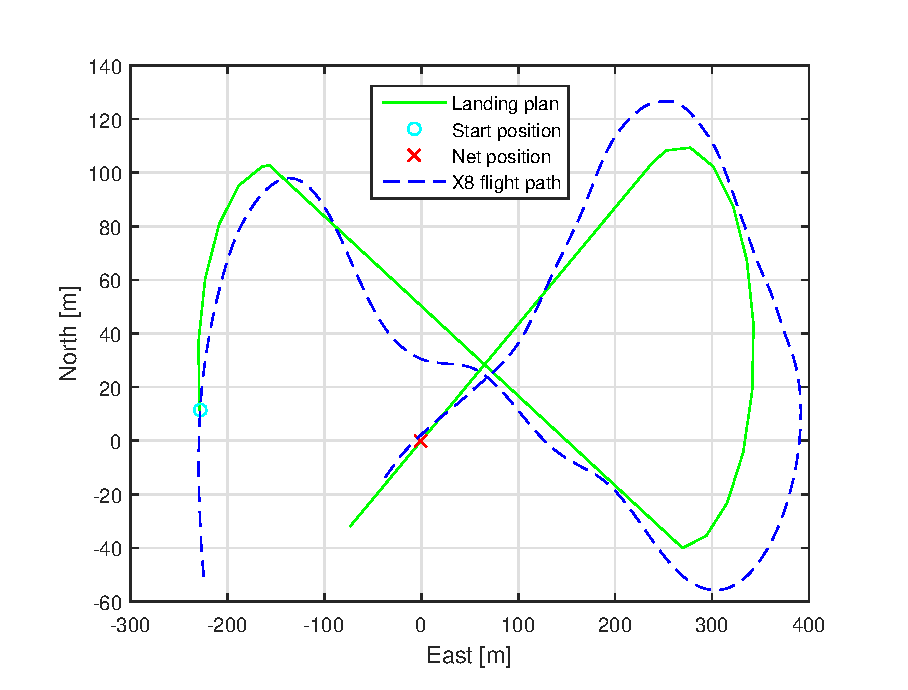
\includegraphics[width=\textwidth]{figs/Experiment/NorthEast31mai103029.eps}
		\caption{North-East plot where the start and finish turning circles have opposite turning directions}
		\label{Fig:NorthEast31mai103029}
\end{subfigure}
\begin{subfigure}{0.7\textwidth}
		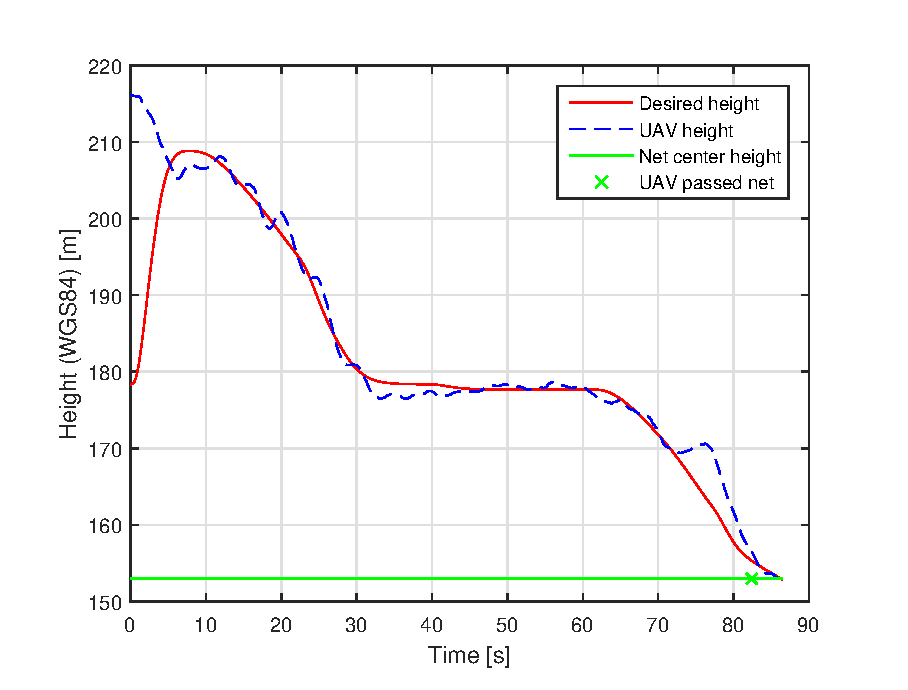
\includegraphics[width=\textwidth]{figs/Experiment/Height31mai103029.eps}
		\caption{Height plot of a landing plan with $3 \deg$ final approach angle}
		\label{Fig:Height31mai103029}
\end{subfigure}
\caption{Test set-up 1}
\label{Fig:Test1}
\end{figure}
%\begin{figure}[H]
%	\centering
%		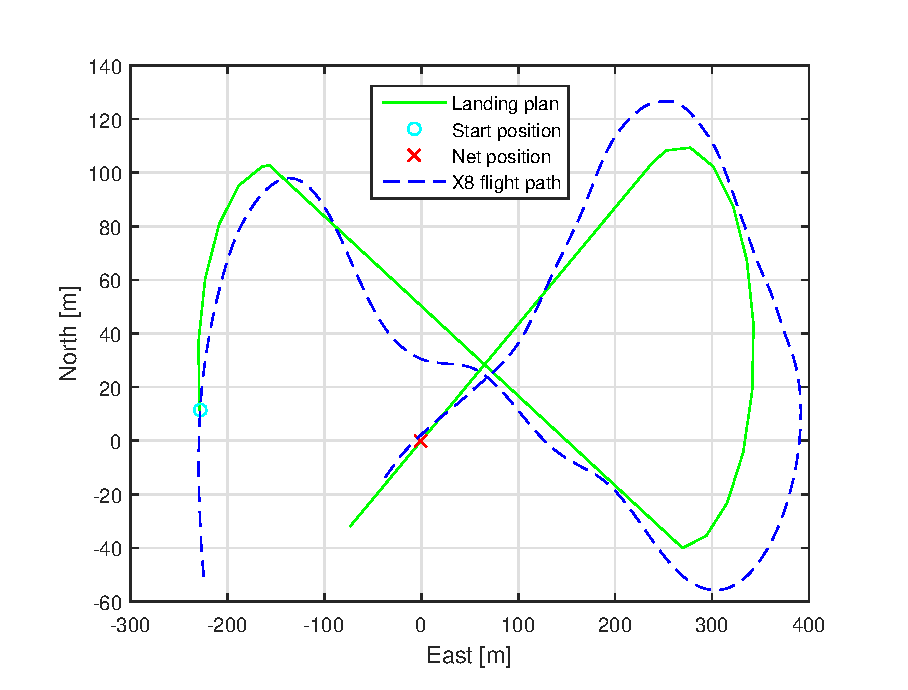
\includegraphics[scale=0.7]{figs/Experiment/NorthEast31mai103029.eps}
%		\caption{North-East plot where the start and finish turning circles have opposite turning directions}
%		\label{Fig:NorthEast31mai103029}
%\end{figure}
%\begin{figure}[H]
%\centering
%		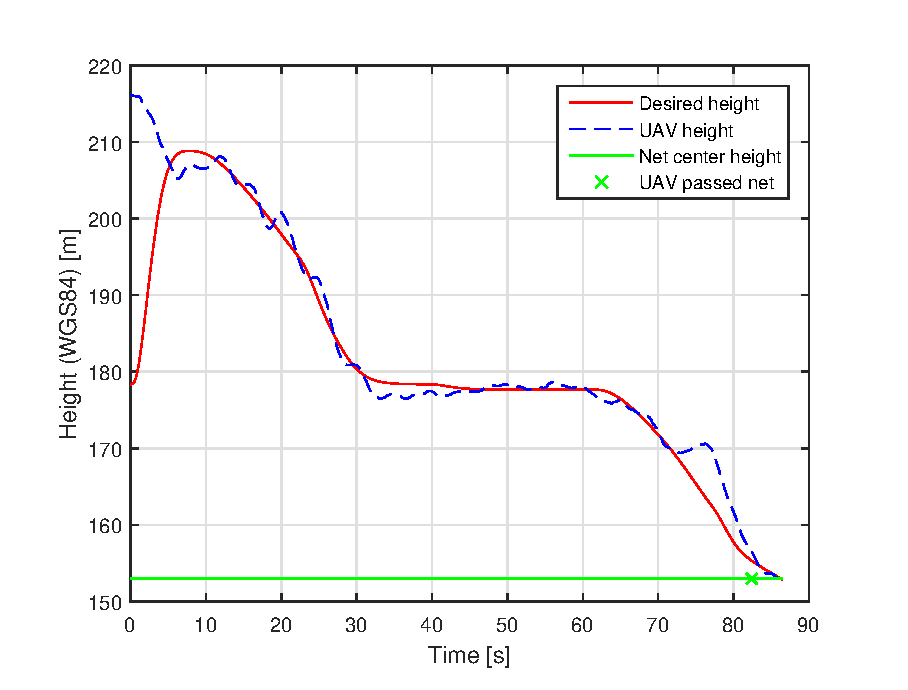
\includegraphics[scale=0.7]{figs/Experiment/Height31mai103029.eps}
%		\caption{Height profile of a landing plan with $3 \deg$ final approach angle}
%		\label{Fig:Height31mai103029}
%\end{figure}
%\subsubsection{Discussion of performance, results and findings}
%The effect of flying in the cross wind introduced oscillatory motion in the \gls{uav}, which the lateral control system was unable to compensate for. The effect of the oscillatory motion affected the \gls{uav} when entering the finish turning circle, where the result was the \gls{uav} overshooting the desired path. The consequence of the \gls{uav} overshooting the finish turning circle can result in the \gls{uav} to leave the line of sight of the pilot, which is a failure when flying in a LOS operation. The \gls{uav} continues to oscillate when flying along the landing path, however the cross track error was within the acceptance criteria listed in table \ref{tb:NetCriteria} at the time the \gls{uav} passed the virtual net.
%
%The longitudinal control system was able to follow it's desired height reference during the approach path, however the \gls{uav} height starts to diverge from the desired height during the landing path. The divergence corresponds to the overshot in the lateral plan, which could be the reason for the divergence. However the desired height from the longitudinal control system was higher then the net center height at the time the \gls{uav} passed the virtual net. The reason behind this behaviour is due to the reference model in the longitudinal control system attempt to create a smooth glide slope towards the aiming waypoint behind the net, which cause the desired height to lag behind the desired path. This behaviour can be removed by setting the final approach angle to zero, thus ensuring that the straight line through the net center has a constant height value.
\subsection{Test set-up 2 - Final approach angle}\label{ss:Day1FinalApp}
\subsubsection{General - Test parameters}
The landing plan parameters used in this test are the same as in section \ref{ss:TestParaInitiDay1}, with the exception of the final approach angle which has been set to $0 \deg$. The goal with this alteration is to ensure the desired height equals the net center height, which will allow the \gls{uav} to converge towards the net center height. The data used to represent this test configuration is retrieved from test number $3$ in table \ref{tb:Day1ParameterAlteration}. Test $3$ is the only one that runs with this configuration.
\subsubsection{Test results and UAV performance}
 The resulting plot of the desired and actual height of the \gls{uav} is shown in figure \ref{Fig:Height31mai31mai105034}, which shows desired height converging to the net center height. Figure \ref{Fig:NorthEast31mai105034} shows a North-East plot of the path created with the new landing plan parameters, which shows significant oscillation along the straight line between the turning circles. The result of the oscillation is a large overshot from the desired path in the finish turning circle.
 \newpage
\begin{figure}[H]
\centering
\begin{subfigure}{0.7\textwidth}
		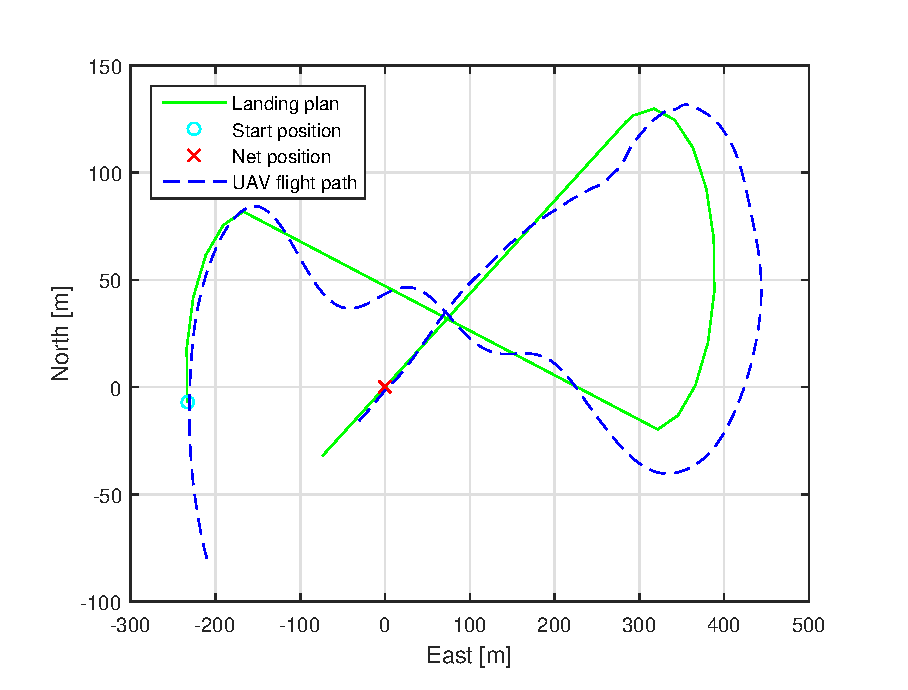
\includegraphics[width=\textwidth]{figs/Experiment/NorthEast31mai105034.eps}
\caption{North-East plot of test set-up 2}
\label{Fig:NorthEast31mai105034}
\end{subfigure}
\begin{subfigure}{0.7\textwidth}
		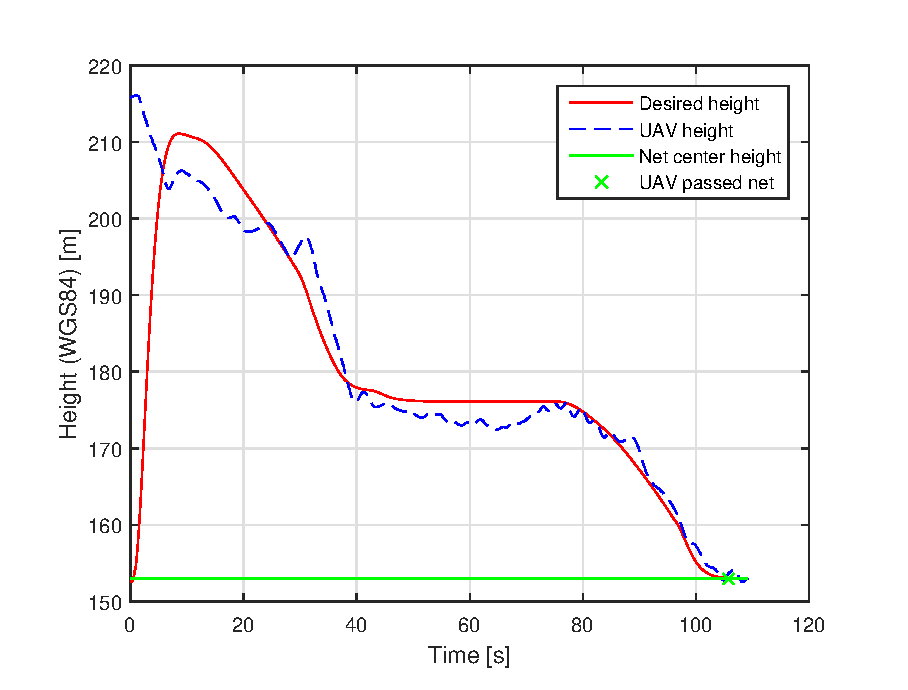
\includegraphics[width=\textwidth]{figs/Experiment/Height31mai105034.eps}
		\caption{Height plot of a landing plan with $0 \deg$ final approach angle}
		\label{Fig:Height31mai31mai105034}
\end{subfigure}
\caption{Test set-up 2}
\label{Fig:Test2}
\end{figure}

%\begin{figure}[H]
%\centering
%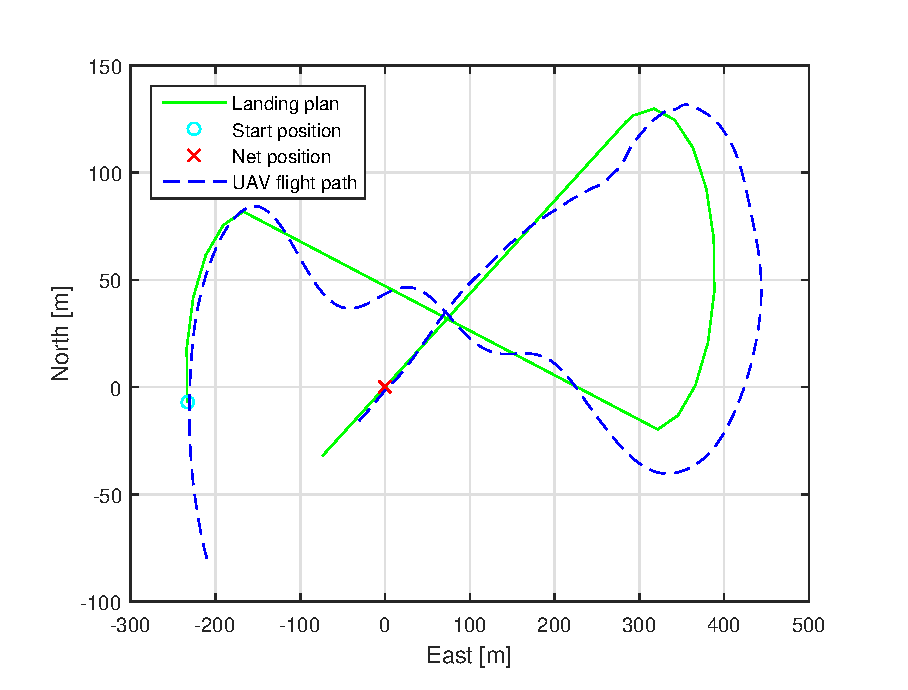
\includegraphics[scale=0.7]{figs/Experiment/NorthEast31mai105034.eps}
%\caption{North-East plot of test set-up 2}
%\label{Fig:NorthEast31mai105034}
%\end{figure}
%\begin{figure}[H]
%\centering
%		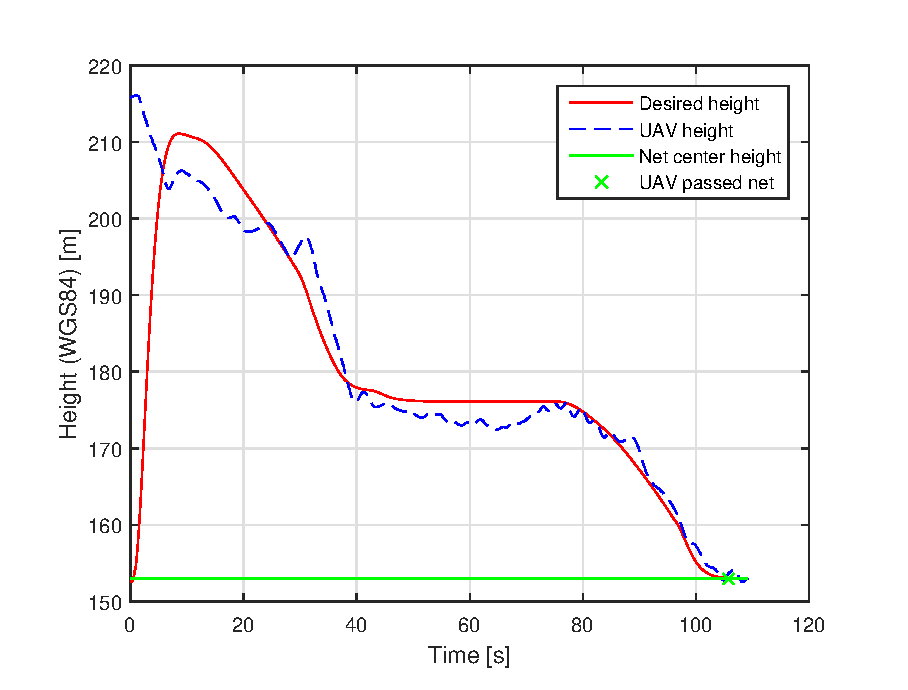
\includegraphics[scale=0.7]{figs/Experiment/Height31mai105034.eps}
%		\caption{Height profile of a landing plan with $0 \deg$ final approach angle}
%		\label{Fig:Height31mai31mai105034}
%\end{figure}
%\subsubsection{Discussion of performance, results and findings}
%The effect of setting the final approach angle to zero gave an increased performance from the longitudinal control system, due to the desired height now converging to the net center height. At the time the \gls{uav} passed the virtual net the hight error with respect the height of the net center was within the height error acceptance.
\subsection{Test set-up 3 - Inverted rotation in start turning circle}\label{ss:Day1Inverted}
\subsubsection{General - Test parameters}
The landing plan parameters used in this test are the same as in section \ref{ss:Day1FinalApp}, with the exception of the rotation direction of the start circle which has been inverted. This will allow a smoother transition between the turning circles, and reduce the duration the \gls{uav} flies in the cross wind. Thus less oscillation is expected and increased performance from the lateral control system. The data used to represent this test configuration is retrieved from test number $4$ in table \ref{tb:Day1ParameterAlteration}. Test $4-9$ were run with this configuration.
\subsubsection{Test results and UAV performance}
A landing plan with the rotation direction of the start turning circle inverted with respect to the previous landing plan, as shown in figure \ref{Fig:NorthEast31mai125420}. The straight line in the approach path allows now for a smoother transition between the two turning circles, and orientate the \gls{uav} into the tail wind. Figure \ref{Fig:Height31mai125420} shows the desired and actual height height of the \gls{uav} together with the net center height. The heigh plot shows that the \gls{uav} follows the desired height and is able to converge to the net center height before passing the net.
\newpage
\begin{figure}[H]
\centering
\begin{subfigure}{0.7\textwidth}
		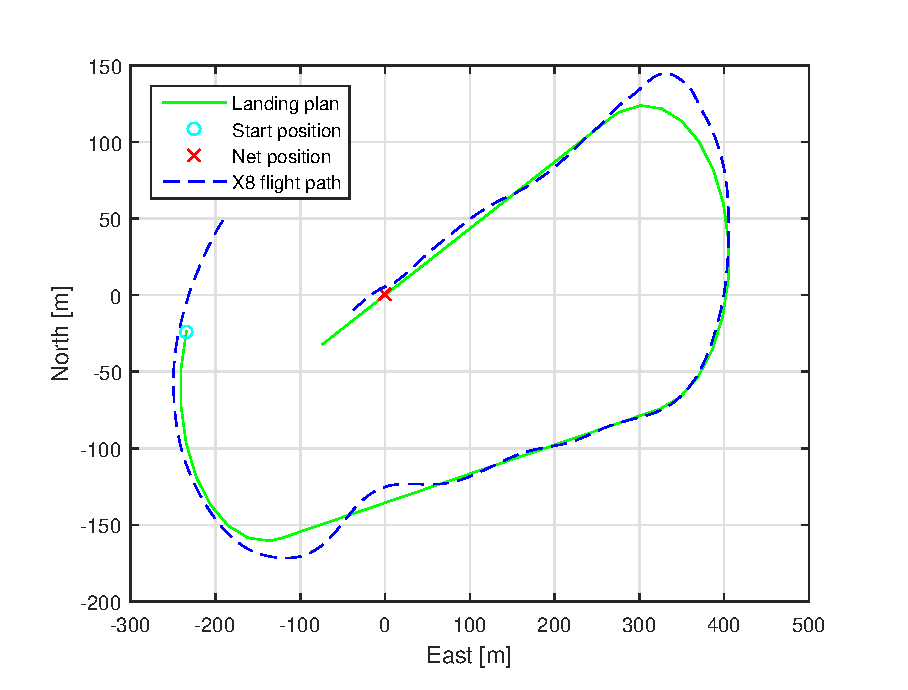
\includegraphics[width=\textwidth]{figs/Experiment/NorthEast31mai125420.eps}
	\caption{North-East plot where the start and finish turning direction have the same turning direction}
	\label{Fig:NorthEast31mai125420}
\end{subfigure}
\begin{subfigure}{0.7\textwidth}
		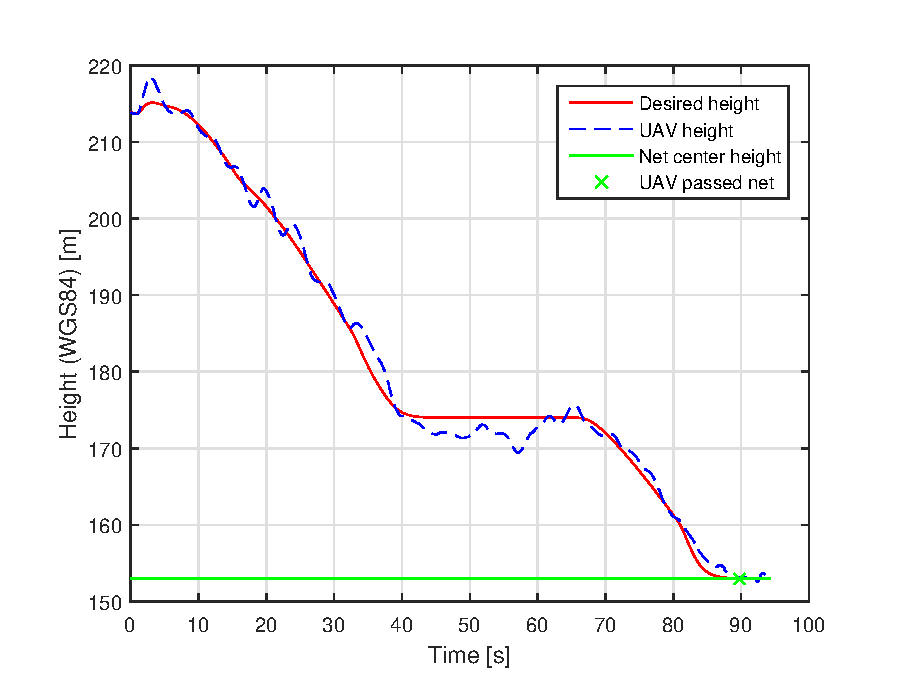
\includegraphics[width=\textwidth]{figs/Experiment/Height31mai125420.eps}
\caption{Height plot for the landing plan test set-up 3}
\label{Fig:Height31mai125420}
\end{subfigure}
\caption{Test set-up 3}
\label{Fig:Test3}
\end{figure}

%\begin{figure}[H]
%	\centering
%	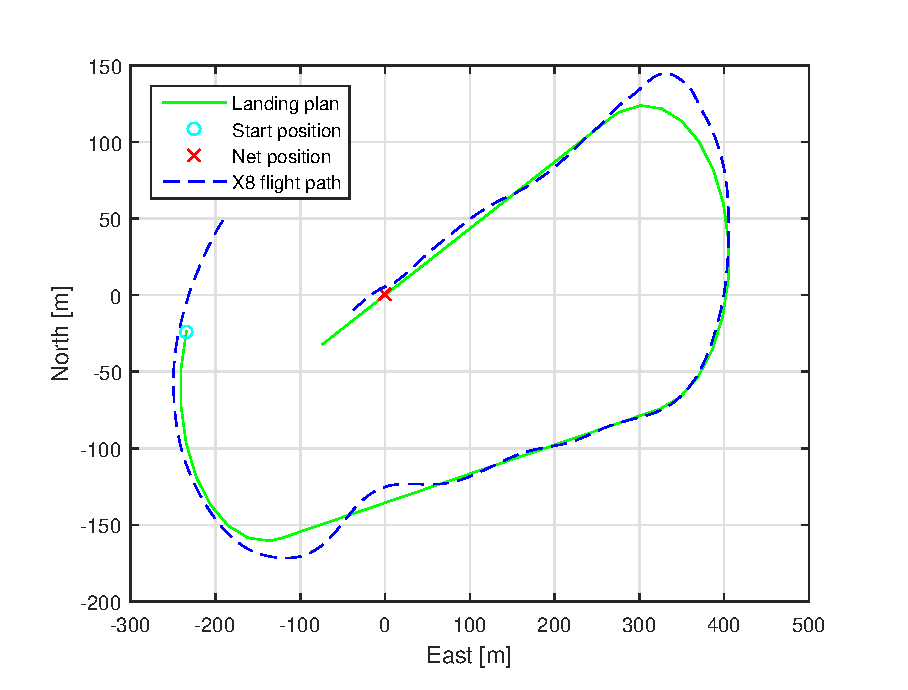
\includegraphics[scale=0.7]{figs/Experiment/NorthEast31mai125420.eps}
%	\caption{North-East plot where the start and finish turning direction have the same turning direction}
%	\label{Fig:NorthEast31mai125420}
%\end{figure}
%\begin{figure}[H]
%\centering
%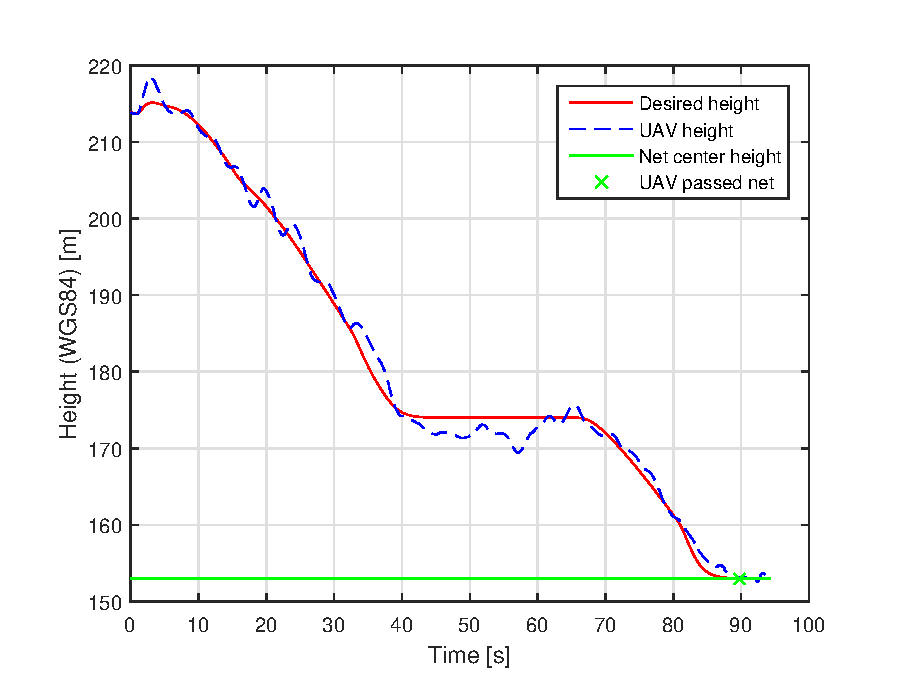
\includegraphics[scale=0.7]{figs/Experiment/Height31mai125420.eps}
%\caption{Height profile for the landing plan test set-up 3}
%\label{Fig:Height31mai125420}
%\end{figure}
%\subsubsection{Discussion of performance, results and findings}
%The result of this alteration was reduced oscillation in the lateral plane for the \gls{uav} when flying along the straight line between the turning circles. The \gls{uav} still experience overshot in the finish turning circle, however the overshooting is reduced due to more stable entry into the finish turning circle.
\subsection{Test set-up 4 - Reduced lateral lookahead distance}\label{ss:Day1:ReducedLookahead}
\subsubsection{General - Test parameters}
The landing plan parameters used in this test are the same as in section \ref{ss:Day1Inverted}, however the lookahead distance in the lateral control system has been reduced from $50$ to $30$. The goal with this alteration is to reduce the oscillatory motion in the lateral plan by making the lateral control system more aggressive when flying in the head wind. The data used to represent this test configuration is retrieved from test number $10$ in table \ref{tb:Day1ParameterAlteration}. Test $10$ and $11$ were run with this configuration.
\subsubsection{Test results and UAV performance}
The effect of this change is shown in figure \ref{Fig:NorthEast31mai131844}, where the oscillatory motion in the lateral plane is almost completely removed. The height plot for test set-up 4 is shown in figure \ref{Fig:Height31mai131844}, which shows that the \gls{uav} is unable to follow the desired height during the final phase of the landing plan.
\newpage
\begin{figure}[H]
\centering
\begin{subfigure}{0.7\textwidth}
		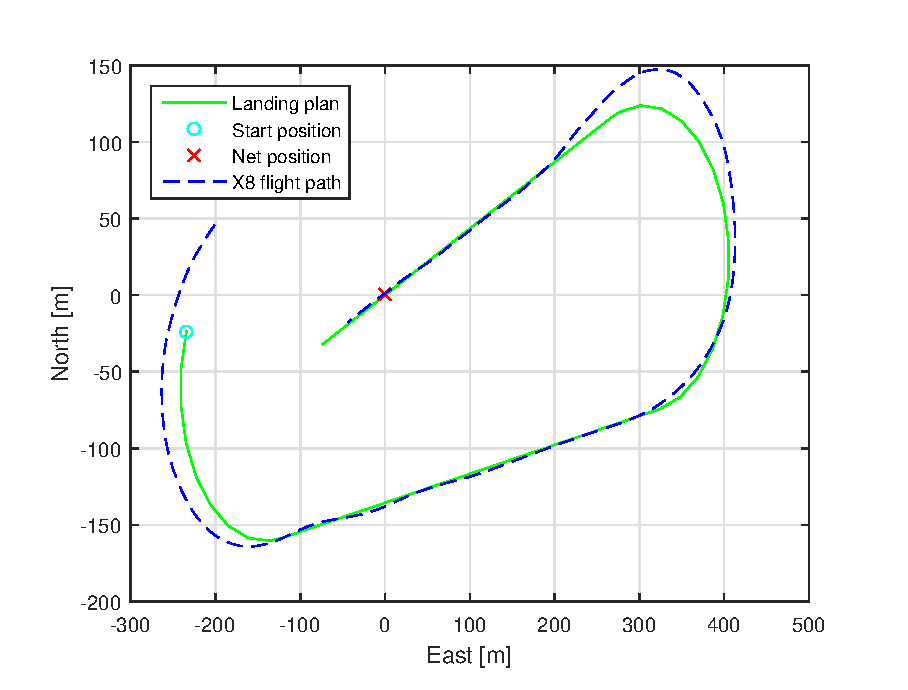
\includegraphics[width=\textwidth]{figs/Experiment/NorthEast31mai131844.eps}
\caption{North-East plot where the lookahead distance of the lateral controller was reduced to increase performance of the autonomous landing system when flying against the wind}
\label{Fig:NorthEast31mai131844}
\end{subfigure}
\begin{subfigure}{0.7\textwidth}
		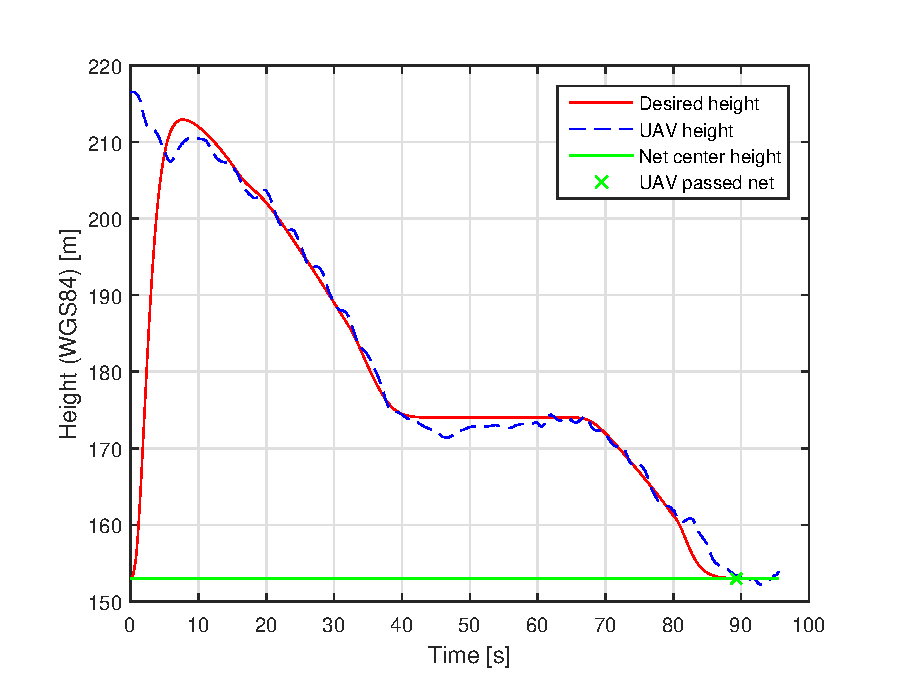
\includegraphics[width=\textwidth]{figs/Experiment/Height31mai131844.eps}
\caption{Height plot for the landing plan test set-up 4}
\label{Fig:Height31mai131844}
\end{subfigure}
\caption{Test set-up 4}
\label{Fig:Test4}
\end{figure}

%\begin{figure}[H]
%\centering
%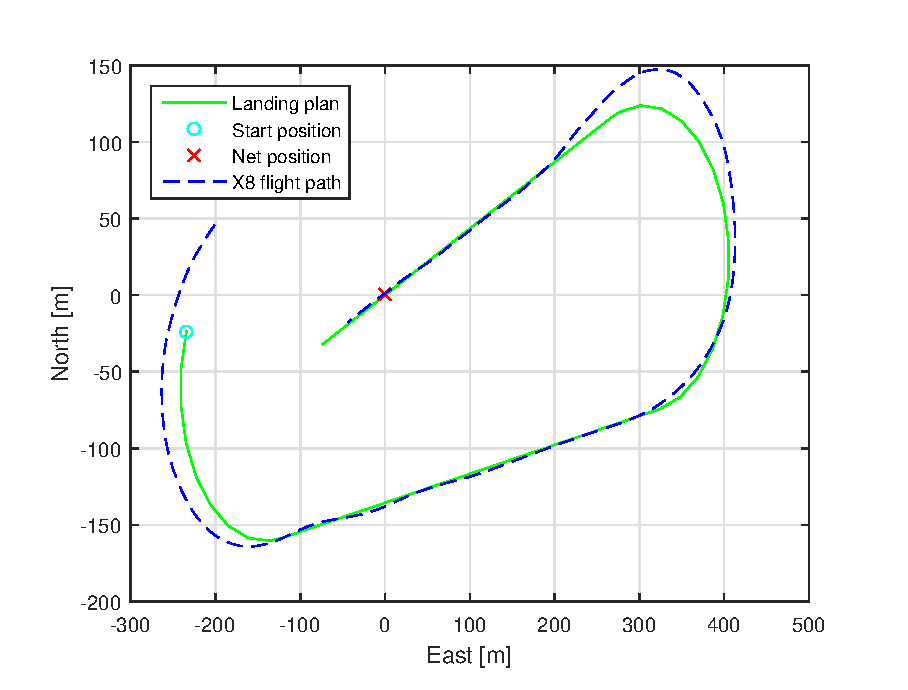
\includegraphics[scale=0.7]{figs/Experiment/NorthEast31mai131844.eps}
%\caption{North-East plot where the lookahead distance of the lateral controller was reduced to increase performance of the autonomous landing system when flying against the wind}
%\label{Fig:NorthEast31mai131844}
%\end{figure}
%\begin{figure}[H]
%\centering
%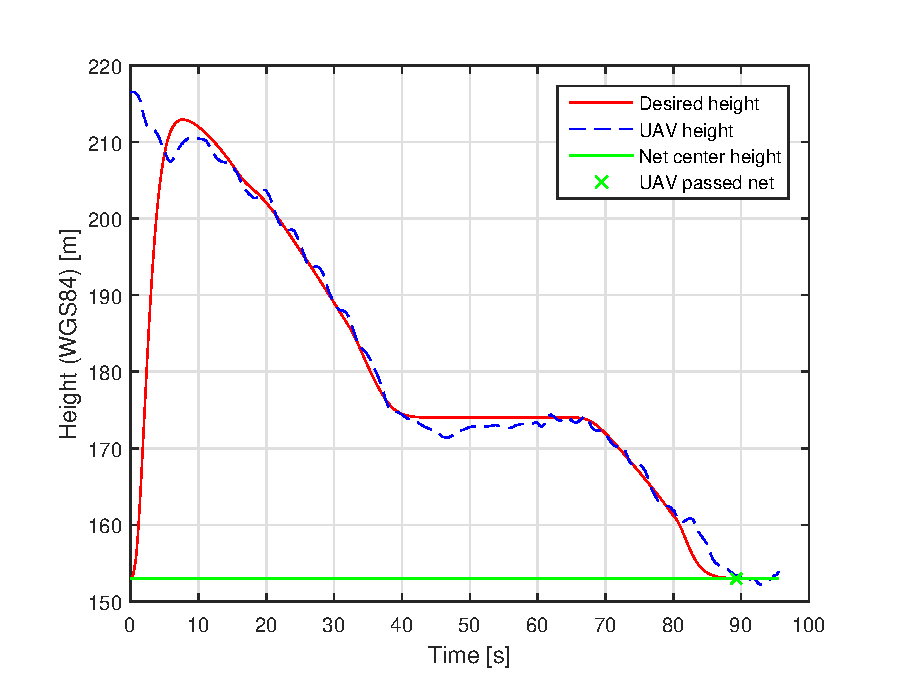
\includegraphics[scale=0.7]{figs/Experiment/Height31mai131844.eps}
%\caption{Height profile for the landing plan test set-up 4}
%\label{Fig:Height31mai131844}
%\end{figure}
%\subsubsection{Discussion of performance, results and findings}
%Reduction of the lookahead distance in the lateral control system resulted in less oscillation in the lateral plane, however the reduced lookahead distance did not affect the overshot in the finish turning circle. In figure \ref{Fig:DesiredRoll131844} was it observed that the lateral control system is reducing its desired roll too early during the turning manoeuvre in the finish turning circle. This happens since the lateral control system only sees the next point on the circle, and not the circle as a whole.
\subsection{Summary of day 1}\label{sss:summaryDay1}
The results from the first day was affected by strong wind condition, in which the \gls{uav} struggled to stay on the desired path. The heigh and cross track error for the 11 landing plan missions performed during the first day are given in table \ref{tb:Day1HeightCrossTrack}. The average height error vary less then the average cross track error, with a variance of $0.4 m$ against $6.2 m$. However the performance of the \gls{uav} in both height error and cross track error is reduced compared to the results obtain during \gls{sil} simulation in section \ref{ss:SILLandingPlan}. The magnitude of the variance in the average cross track error shows that the performance of the lateral control system should be further improved for the autonomous landing system to be considered reliable.
\begin{table}[H]
\centering
\begin{tabular}{| l | l | l |}
\hline
\textbf{Test Nr.} 	& \textbf{Average height error [m]} 	& \textbf{Average cross track error [m]}  \\ \hline
$1$				& $1.5$							& $6.1$								\\ \hline
$2$				& $2.6$							& $6.7$								\\ \hline
$3$				& $0.9$							& $5.5$								\\ \hline
$4$				& $0.1$							& $2.8$								\\ \hline
$5$				& $1.7$							& $2.0$								\\ \hline
$6$				& $1.3$							& $6.8$								\\ \hline
$7$				& $1,8$							& $9.1$								\\ \hline
$8$				& $1.2$							& $8.2$								\\ \hline
$9$				& $1.9$							& $5.9$								\\ \hline
$10$			& $1.5$							& $4.4$								\\ \hline
$11$			& $1.5$							& $1.4$								\\ \hline \hline
Average			& $1.5$							& $5.4$								\\ \hline
Variance		& $0.4$							& $6.2$								\\ \hline
\end{tabular}
\caption{Average height and cross track error from the first day of testing}
\label{tb:Day1HeightCrossTrack}
\end{table}
The variance of the longitudinal control system shows reliable in performance, but the average error should be reduced in order for the autonomous landing system to be able to hit the stationary net with increased probability of success. The results of whether or not the \gls{uav} was within the net acceptance criteria at the time of net passing, is given in table \ref{tb:Day1LandingAttempt}. The alteration of the path and controller parameters mostly aimed towards the lateral control system, resulting in reduced average error from the later tests. In comparison to the \gls{sil} simulation results, where the average cross track error was almost zero, the performance has clearly decreased. This behaviour was expected due the simulation model used in the simulation has not been verified, in addition to better tuned controllers in the \gls{sil} simulator.
\begin{table}[H]
\centering
\begin{tabular}{| p{0.5cm} | p{1cm} | p{1cm} | p{3.5cm} | p{3cm} | p{1cm} |}
\hline
\textbf{Test Nr.}	& \textbf{Height error [m]}	& \textbf{Cross track error [m]}& \textbf{Height acceptance}& \textbf{Cross track error acceptance}	& \textbf{Net hit}\\ \hline
$1$				& $2.8$		& $2.1$		& X								& OK									& X					\\ \hline
$2$				& $2.7$		& $-4.5$	& X								& X										& X					\\ \hline
$3$				& $0.9$		& $-1.6$	& OK							& OK									& OK				\\ \hline
$4$				& $0.0$		& $5.4$		& OK							& X										& X					\\ \hline
$5$				& $0.8$		& $5.3$		& OK							& X										& X					\\ \hline
$6$				& $2.1$		& $-1.6$	& X								& OK									& X					\\ \hline
$7$				& $0.7$		& $2.3$		& OK							& OK									& OK				\\ \hline
$8$				& $-1.5$	& $-5.4$	& X								& X										& X					\\ \hline
$9$				& $1.9$		& $0.8$		& X								& OK									& X					\\ \hline
$10$			& $0.3$	& $1.1$		& OK							& OK									& OK				\\ \hline
$11$			& $-1.3$	& $0.2$		& OK							& OK									& OK				\\ \hline
\end{tabular}
\caption{Net passing result from the first day of testing. The acceptance criteria used to determine if the \gls{uav} passed through the net is given in table \ref{tb:NetCriteria}}
\label{tb:Day1LandingAttempt}
\end{table}
The content of table \ref{tb:Day1LandingAttempt} is shown in figure \ref{Fig:Day1NetPass}, where the net is marked as a whole line and all the tests from the first day are marked as crosses. The oscillatory motion in the lateral plane by the \gls{uav} is reflected in the placement of the crosses. The placement of the cross shows the effect of an high average height error by either passing over the net or in the upper part of the net.
\newpage
\begin{figure}[H]
\centering
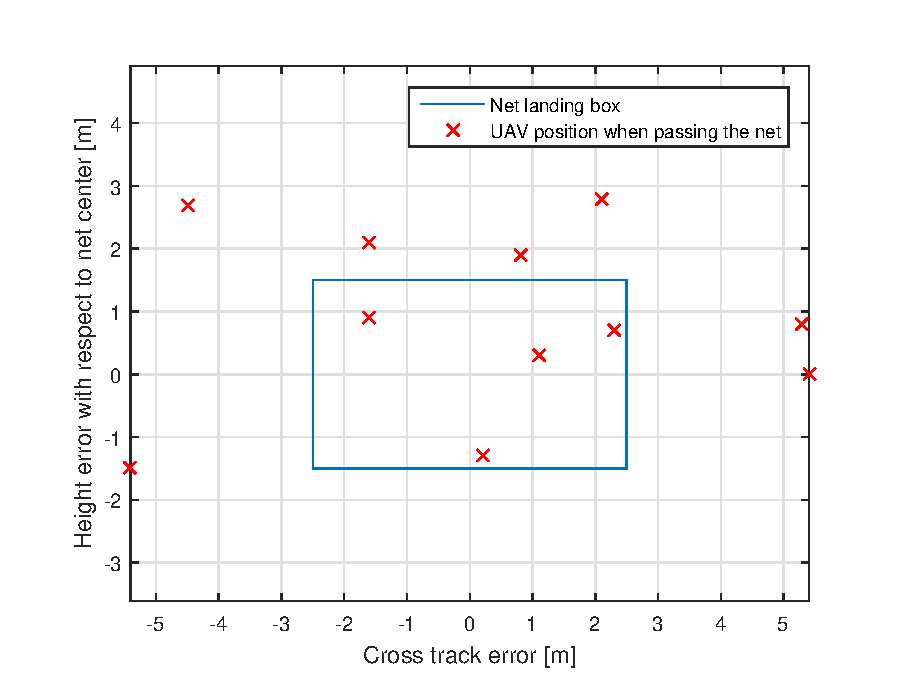
\includegraphics[scale=0.7]{figs/Experiment/day1NetHit.eps}
\caption{Position of \gls{uav} relative to the net center at the time of net passing}
\label{Fig:Day1NetPass}
\end{figure}
%During the execution of the landing plans it was discovered that in order for the \gls{uav} to stay above the highest tree tops it had to start its decent from an altitude of $56 m$ above the airfield. Flying bellow this height would result in the pilot losing sight of the \gls{uav}, which is unacceptable in a LOS \gls{uav} operation. This didn't provide a problem during landing attempt with a virtual net which was placed $26 m$ above the airfield, however during a real stationary net landing it would push the limitation of the operation area in which the \gls{uav} can fly. A $56 m $ decent with a glide slope angle of $6\deg$ would require a glide slope of $500 m$. An estimate of the the available length of which the \gls{uav} can use for autonomous landing in a stationary net is estimated to be $700 m$. This would require the use of the entire runway at Agdenes. An alternative solution is to attempt to land with a greater glide slope angle, or simply start the landing path from the west with respect to the runway. Landing attempts from the west has yet to tried, the reason being limited time and that the \gls{uav} would have to land in tail wind, which would result in a less stable performance from the lateral control system during windy condition.
\section{Execution of testing - Day 2 (Calm condition)}
\subsection{Performed tests}
A total number of 8 test flights were conducted during the second day of testing. During these tests two different configuration were tested. The different test configurations includes increased glide slope angle and reduced distance between arc segments in the turning circles. Table \ref{tb:Day2ParameterAlteration} list up the number of flight test which was perform during the second day, in addition to the state of the autonomous landing system parameter which was altered in one of the two different configuration set-ups. Test number $1,2,6,7$ and $8$ were test with increased glide slope angle and test number $3-5$ were test with reduced arc segment distance. Only test configuration number $1$ and $5$ are presented in plots, while all test data are used to determine the overall performance of the autonomous landing system during the second day.
\begin{table}[H]
\centering
\begin{tabular}{| p{0.5cm} | p{3cm} | p{4cm} |}
\hline
\textbf{Test Nr.} & \textbf{Glide slope angle [deg]} &  \textbf{Turning arc segment distance [m]}\\ \hline
$1$				& $8$ & $ 25 $		\\ \hline
$2$				& $6$ & $ 25 $		\\ \hline
$3$				& $6$ & $ 10 $		\\ \hline
$4$				& $6$ & $ 10 $		\\ \hline
$5$				& $6$ & $ 10 $			\\ \hline
$6$				& $7$ & $ 10 $		\\ \hline
$7$				& $6$ & $ 10 $			\\ \hline
$8$				& $6.5$ & $ 10 $	\\ \hline
\end{tabular}
\caption{Table containing the landing plan mission during day 2, with the corresponding state of the parameters altered during the landing plan missions.}
\label{tb:Day2ParameterAlteration}
\end{table}
\subsubsection{Weather condition}
The second day had calm wind condition, considered as ideal field test conditions for the autonomous landing system.
\subsection{Test set-up 5 - Increased glide slope angle}\label{ss:Day2GlideSlope}
\subsubsection{General - Test parameters}
The test set-up 5 parameters were as per those used in test set-up 4 in section \ref{ss:Day1:ReducedLookahead} with the exception of glide slope length and angle which was altered to $280 m$ opposed to $220 m$ and $8 \deg$ opposed to $6 \deg$ respectfully. The full list of landing plan parameter used in this test is given in table \ref{AP:SpecDay2}. Otherwise the autonomous landing system parameters remain unchanged from the parameters used in section \ref{ss:Day1:ReducedLookahead}. The data used to represent this test configuration is retrieved from test number $1$ in table \ref{tb:Day2ParameterAlteration}. Test $1,2,6,7$ and $8$ were run with this configuration.
\subsubsection{Test results and UAV performance}
Figure \ref{Fig:NorthEast1juni081328} shows a North-East plot of the path created with the new landing plan parameters, which show the lateral path overshoots both the start and finish turning circles. The desired height and the actual heigh of the \gls{uav} is shown in figure \ref{Fig:Height1juni081328}, which shows that the \gls{uav} is unable to follow a glide slope with a slope angle of $\gamma_l = 8 \deg$. 

\begin{figure}[H]
\centering
\begin{subfigure}{0.7\textwidth}
		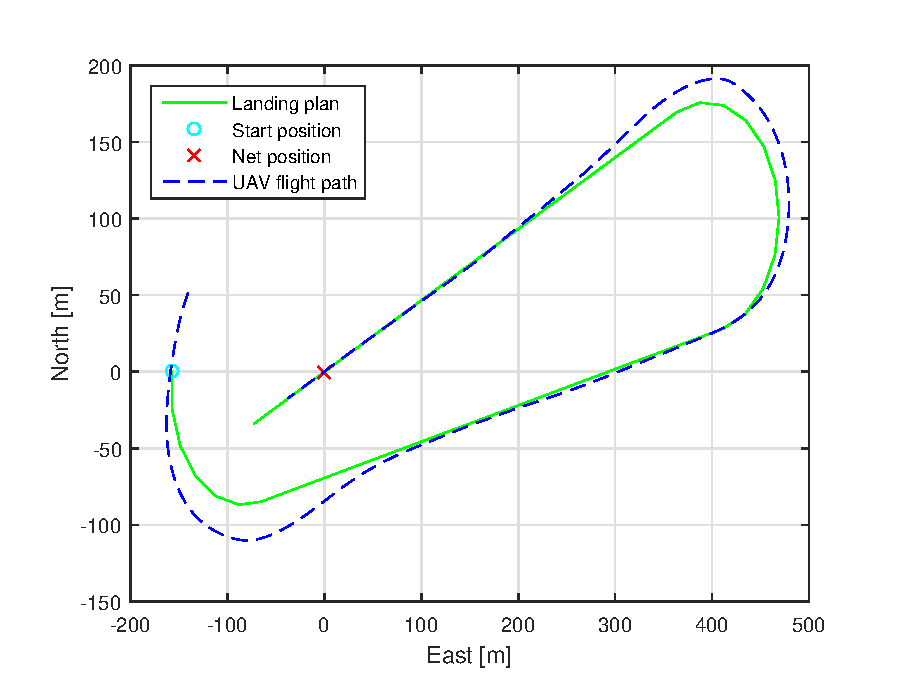
\includegraphics[width=\textwidth]{figs/Experiment/NorthEast1juni081328.eps}
\caption{North-East plot created with the path parameter listed in table \ref{AP:SpecDay2}}
\label{Fig:NorthEast1juni081328}
\end{subfigure}
\begin{subfigure}{0.7\textwidth}
		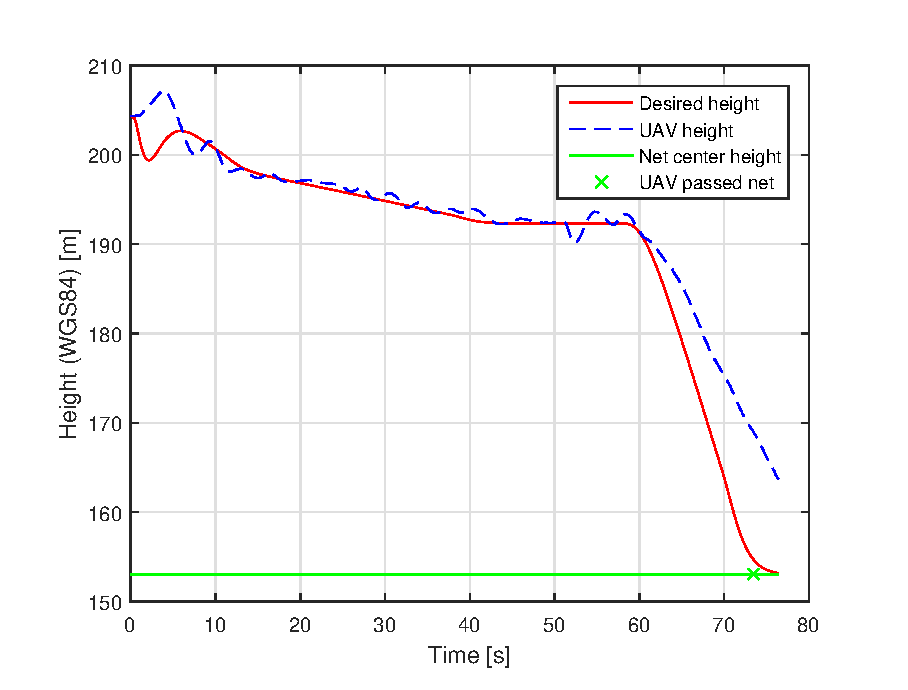
\includegraphics[width=\textwidth]{figs/Experiment/Height1juni081328.eps}
\caption{Desired and actual height of the \gls{uav} with a glide slope angle of $\gamma_l = 8 \deg$}
\label{Fig:Height1juni081328}
\end{subfigure}
\caption{Test set-up 5}
\label{Fig:Test5}
\end{figure}

%\begin{figure}[H]
%\centering
%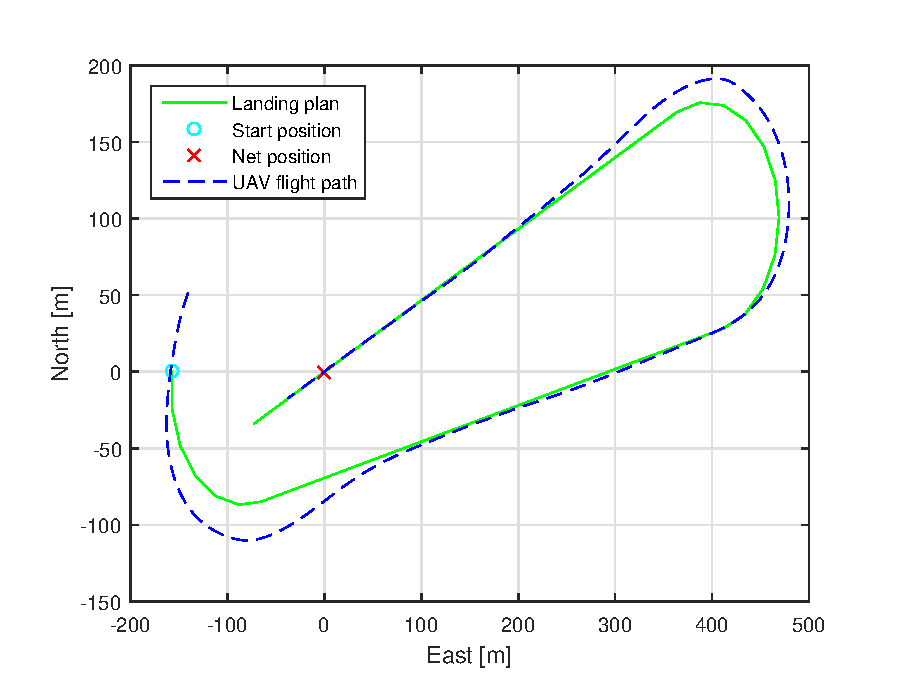
\includegraphics[scale=0.7]{figs/Experiment/NorthEast1juni081328.eps}
%\caption{North-East plot created with the path parameter listed in table \ref{AP:SpecDay2}}
%\label{Fig:NorthEast1juni081328}
%\end{figure}
%The desired height and the actual heigh of the \gls{uav} is shown in figure \ref{Fig:Height1juni081328}, which shows that the \gls{uav} is unable to follow a glide slope with a slope angle of $\gamma_l = 8 \deg$. 
%\begin{figure}[H]
%\centering
%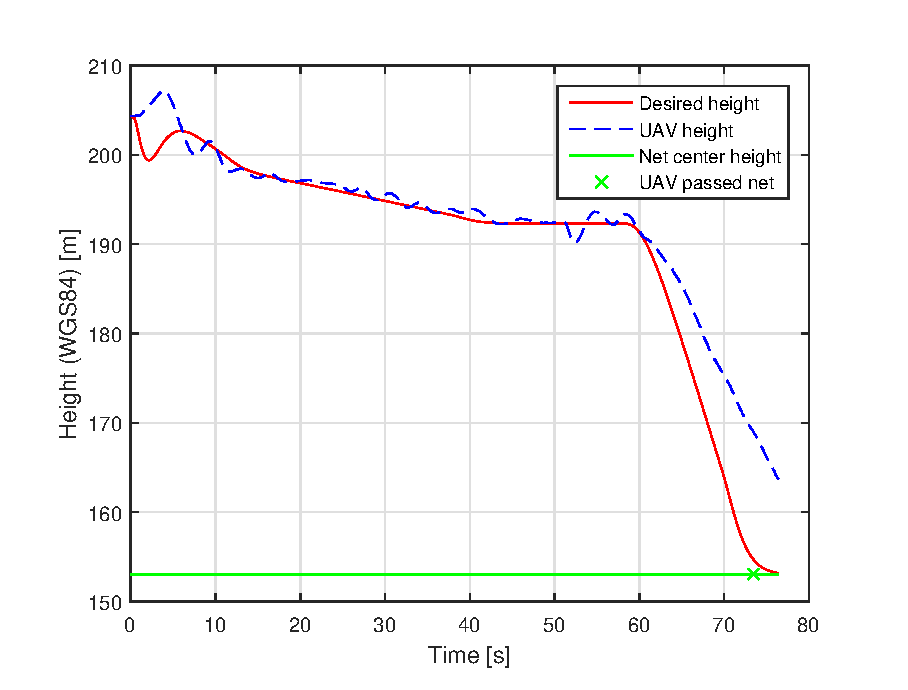
\includegraphics[scale=0.7]{figs/Experiment/Height1juni081328.eps}
%\caption{Desired and actual height of the \gls{uav} with a glide slope angle of $\gamma_l = 8 \deg$}
%\label{Fig:Height1juni081328}
%\end{figure}
%\subsubsection{Discussion of performance, results and findings}
%The longitudinal control system was unable to follow a $8 \deg$ steep glide slope, which was due to the low level pitch controller inability to follow the desired pitch. The low level pitch controller must be further fine tuned, and similar to the low level roll controller, has not been fine tuned for autonomous flights where high precision performance is desired.
%
%The reason for the overshoot in the start tuning circle is due to the low level roll controller being poorly tuned for autonomous flights where high precision performance from the \gls{uav} is desired. In addition the control surface used to control the roll of the \gls{uav} is also used to control the pitch, which results in having to weight the performance in heading against the ability to follow a height reference.
\subsection{Test set-up 6 - Reduced arc segments distance}\label{ss:Day2ArcDistance}
\subsubsection{General - Test parameters}
The landing plan parameters used in this test are the same as in section \ref{ss:Day2GlideSlope}, with the exception of the glide slope angle which has been reduced to $6 \deg$. In an attempt to further reduce the overshoot in the finish turning circle the distance between each arc segments in the approach path circles was reduced from $25 m$ to $10 m$. The desired response with this alteration of the approach path was to ensure that the lateral control system keeps a high desired roll angle through the turning circle, thus reducing the overshoot and increase the performance. The data used to represent this test configuration is retrieved from test number $5$ in table \ref{tb:Day2ParameterAlteration}.
\subsubsection{Test results and UAV performance}
A North-East plot of the resulting path is shown in figure \ref{Fig:NorthEast1juni083423}, which shows that the \gls{uav} reduced its overshot in the final turning circle. The height plot for test set-up 6 is shown in figure \ref{Fig:Height1juni083423}, which shows that the \gls{uav} is able to follow the desired height.
\newpage
\begin{figure}[H]
\centering
\begin{subfigure}{0.7\textwidth}
		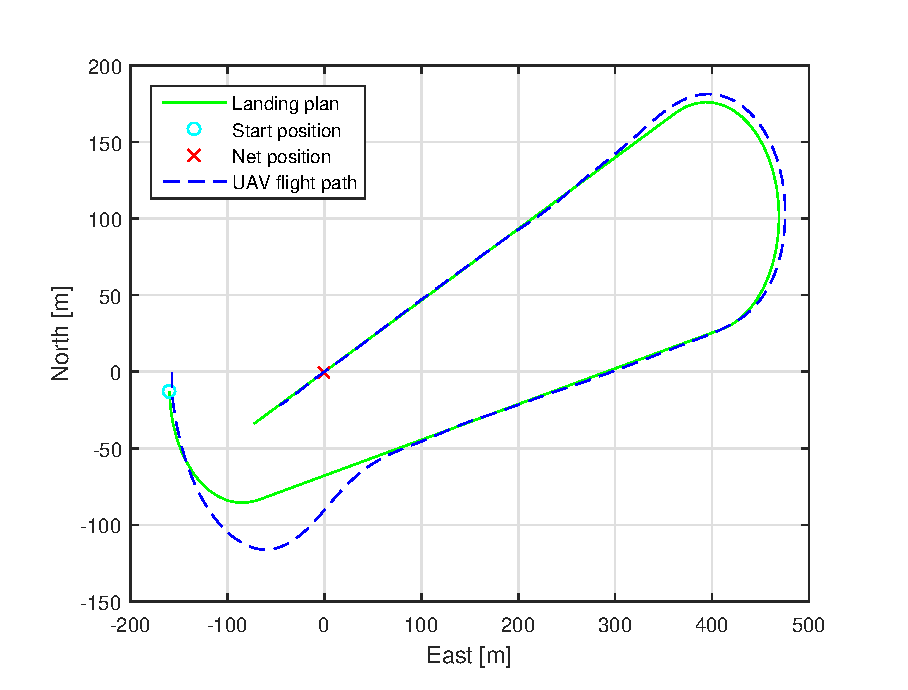
\includegraphics[width=\textwidth]{figs/Experiment/NorthEast1juni083423.eps}
\caption{North-East plot where the distance between each arc segments has been reduced from $25 m$ to $10 m$}
\label{Fig:NorthEast1juni083423}
\end{subfigure}
\begin{subfigure}{0.7\textwidth}
		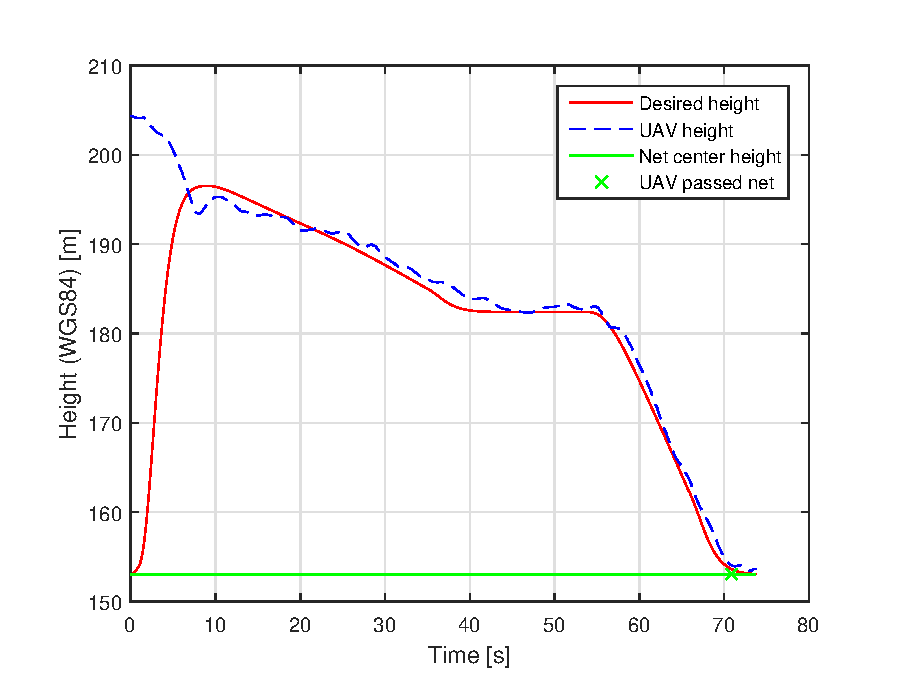
\includegraphics[width=\textwidth]{figs/Experiment/Height1juni083423.eps}
\caption{Heigh plot for landing plan test set-up 6}
\label{Fig:Height1juni083423}
\end{subfigure}
\caption{Test set-up 6}
\label{Fig:Test6}
\end{figure}

%\begin{figure}[H]
%\centering
%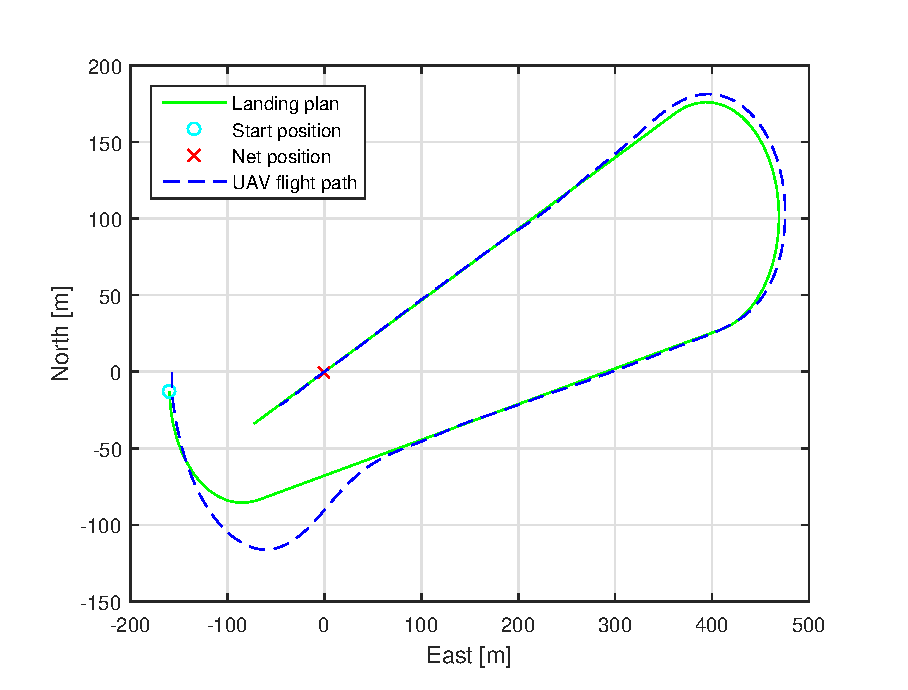
\includegraphics[scale=0.7]{figs/Experiment/NorthEast1juni083423.eps}
%\caption{North-East plot where the distance between each arc segments has been reduced from $25 m$ to $10 m$}
%\label{Fig:NorthEast1juni083423}
%\end{figure}
%\begin{figure}[H]
%\centering
%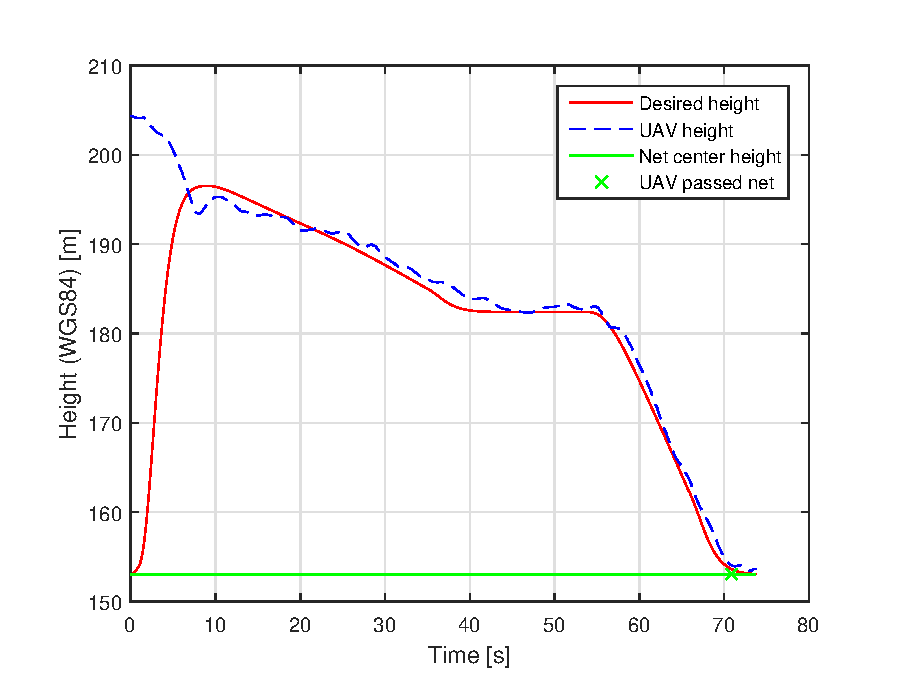
\includegraphics[scale=0.7]{figs/Experiment/Height1juni083423.eps}
%\caption{Heigh profile for landing plan test set-up 6}
%\label{Fig:Height1juni083423}
%\end{figure}
%\subsubsection{Discussion of performance, results and findings}
%The reduced overshot in the finish turning circle shows that a reduced distance between arc segment can be used to achieve a prolonged high desired roll from the lateral control system, which was observed in figure \ref{Fig:RollFinalTurning083423}.
\subsection{Summary of day 2}\label{ss:SummaryDay2}
%%% Bruk som mal
%The result from the first day was affected by strong wind condition, in which the \gls{uav} struggled to stay on the path. The heigh and cross track error for the 11 landing plan missions performed during the first day are given in table \ref{tb:Day1HeightCrossTrack}. The average height error vary less then the average cross track error, with a variance of $0.4 m$ against $6.2 m$. However the performance of the \gls{uav} in both height error and cross track error is worse then the results obtain during SIL simulation in section \ref{ss:SILLandingPlan}.
The weather condition during the second day can be considered ideal for testing the autonomous landing system, thus possible to identify the strength and weaknesses of the system where the weather affect is negligible.

The lateral control system perform better compared to the first day during calm wind condition which is reflected in the table \ref{Tb:AverageCrossHeightDay2}, where the performance from 8 landing plan missions is presented. The performance from the longitudinal control system remain similar to the first day, which shows that the longitudinal control system is less affected by the wind conditions then the lateral control system.
\begin{table}[H]
\centering
\begin{tabular}{| l | l | l |}
\hline
\textbf{Test Nr.} 	& \textbf{Average height error [m]} 	& \textbf{Average cross track error [m]}  \\ \hline
$1$				& $2.2$							& $3.8$										\\ \hline
$2$				& $1.2$							& $3.4$										\\ \hline
$3$				& $0.9$							& $-1.8$									\\ \hline
$4$				& $2.5$							& $-0.2$									\\ \hline
$5$				& $3.0$							& $0.3$										\\ \hline
$6$				& $1.6$							& $0.2$										\\ \hline
$7$				& $1,9$							& $-2.3$									\\ \hline
$8$				& $1.9$							& $-0.1$									\\ \hline \hline
Average			& $1.9$							& $0.5$										\\ \hline
Variance		& $0.5$							& $4.7$										\\ \hline
\end{tabular}
\caption{Average height and cross track error from day 2}
\label{Tb:AverageCrossHeightDay2}
\end{table}
The main objective second day of testing was to increase the height from which the \gls{uav} would start its decent towards the net by increasing the glide slope angle, and to investigate path parameter that can be used to reduce the overshot during turning in the finish turning circle. The attempts to increase the glide slope angle during landing plan mission are reflected in table \ref{tb:Day2LandingAttempt}, which contain the results of whether or not the \gls{uav} passed through the net. Attempts with glide slope angles greater then $6 \deg$ resulted in the \gls{uav} overshooting the net.

%Attempts with glide slope angles greater then $6 \deg$ resulted in the \gls{uav} to overshot the net, however the performance from the longitudinal control system could be increased with a better better tuning of the low level pitch controllers. With the current longitudinal control system the maximum glide slope angle which the X8 is able to follow during a autonomous landing is $6 \deg$. In addition increased performance from the longitudinal control system can be achieved by increasing the length of the final approach, in order for the \gls{uav} to have longer time to converge to the net center height. The final approach length could be increased to $120 m$ by moving the net to the edge of the runway at Agdenes. The risk with a large final approach during a autonomous landing in a real net would be the prolonged time the \gls{uav} flies $3-4 m$ above ground. A loss of high accurate positioning system could then result in a crash.

\begin{table}[H]
\centering
\begin{tabular}{| p{0.5cm} | p{1cm} | p{1cm} | p{3.5cm} | p{3cm} | p{1cm} |}
\hline
\textbf{Test Nr.}	& \textbf{Height error [m]}	& \textbf{Cross track error [m]}& \textbf{Height acceptance}& \textbf{Cross track error acceptance}	& \textbf{Net hit}\\ \hline
$1$				& $14.4$		& $0.1$		& X								& OK									& X					\\ \hline
$2$				& $1.3$		& $0.6$	& OK								& OK										& OK					\\ \hline
$3$				& $1.1$		& $-0.2$	& OK							& OK									& OK				\\ \hline
$4$				& $1.4$		& $0.1$		& OK							& OK										& OK					\\ \hline
$5$				& $1.1$		& $0.1$		& OK							& OK										& OK					\\ \hline
$6$				& $2.0$		& $-0.2$	& X								& OK									& X					\\ \hline
$7$				& $2.3$		& $0.2$		& X								& OK									& X				\\ \hline
$8$				& $7.0$	& $0.3$			& X										& OK										& X					\\ \hline
\end{tabular}
\caption{Net passing result from the second day of testing. The acceptance criteria used to determine if the \gls{uav} passed through the net is given in table \ref{tb:NetCriteria}}
\label{tb:Day2LandingAttempt}
\end{table}
The high average height error of the longitudinal control system is reflected in figure \ref{Fig:Day2NetPass}, where those crosses that are within the height acceptance criteria are in the upper part of the net.
\begin{figure}[H]
\centering
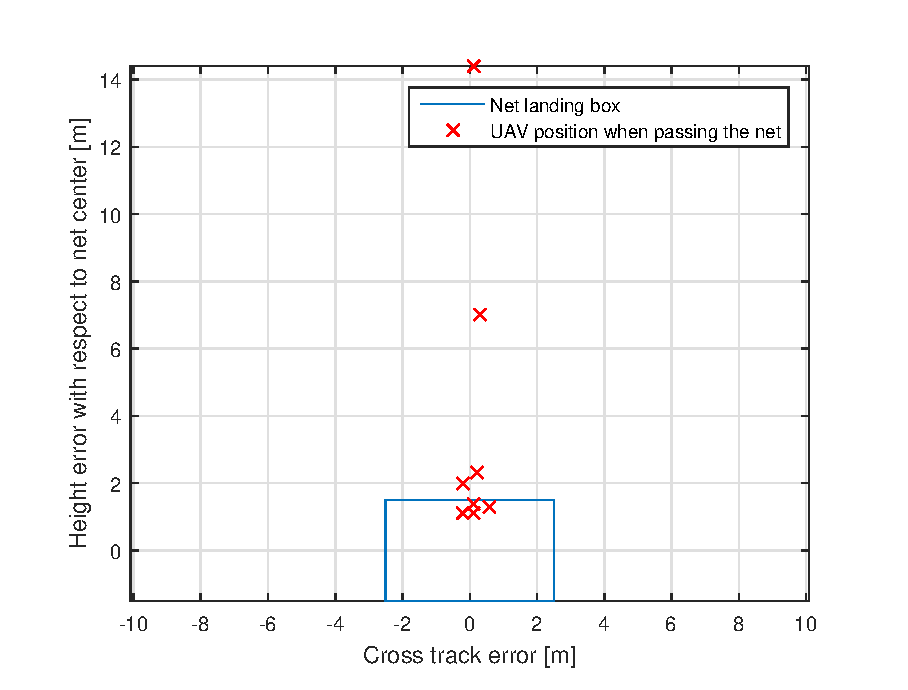
\includegraphics[scale=0.7]{figs/Experiment/day2NetHit.eps}
\caption{Position of the \gls{uav} relative to the net center at the time of net passing}
\label{Fig:Day2NetPass}
\end{figure}
\section{Navigation system performance}\label{ss:NavigationResults}
\subsection{RTK-GNSS performance}
The performance from the \gls{rtk-gnss} system during both days of testing the autonomous landing system resulted in similar performance, thus only results from the first day is presented in this section, while the results from the second day is given in appendix \ref{AP:ADDResults}. The results from the \gls{rtk-gnss} system during the landing plan flights is summarised in table \ref{TB:RTKFirstDayRTK}, where the result is presented as percentage of the total number of GpsFixRtk \gls{imc} messages.
\begin{table}[H]
\centering
\begin{tabular}{| l | l | l | l |}
\hline
\textbf{Test Nr.}	& \textbf{FIX \%}	& \textbf{FLOAT \%}	& \textbf{NONE \%}	\\ \hline
$1$				& $99.5 $	& $0.5$	& $0.0$									\\ \hline
$2$				& $99.5 $	& $0.5$	& $0.0$									\\ \hline
$3$				& $99.8 $	& $0.0$	& $0.0$									\\ \hline
$4$				& $100$		& $0.0$	& $0.0$									\\ \hline
$5$				& $100$		& $0.0$	& $0.0$									\\ \hline
$6$				& $100$		& $0.0$	& $0.0$									\\ \hline
$7$				& $99.9$	& $0.1$	& $0.0$									\\ \hline
$8$				& $99.7 $ 	& $0.3$	& $0.0$									\\ \hline
$9$				& $99.3$	& $0.7$	& $0.0$									\\ \hline
$10$			& $100$		& $0.0$	& $0.0$									\\ \hline
$11$			& $100$		& $0.0$	& $0.0$									\\ \hline
\end{tabular}
\caption{Performance of the \gls{rtk-gnss} system the first day during the executing of the landing plans}
\label{TB:RTKFirstDayRTK}
\end{table}
\subsection{Short loss compensator}
The short loss compensator was engaged during a flight where the \gls{rtk-gnss} started to experience problem. The flight plan was part of cooperative net recovery system presented in \citep{Sigurd} and \citep{Jostein}, which experience reduced \gls{rtk-gnss} performance due to decreased satellite geometry. During the flight the \gls{rtk-gnss} system experienced a drop out, as seen in figure \ref{Fig:NavSource}. The main reason for the drop out is shown in figure \ref{Fig:SatCount1juni114124}, where at the time of \gls{rtk-gnss} drop out the number of valid satellites starts to vary rapidly. Even though the \gls{rtk-gnss} position solution is unavailable the navigation system is still able to supply high accurate position solution due to the short \gls{rtk-gnss} compensator as seen in figure \ref{Fig:ShortLoss}.
\begin{figure}[H]
\centering
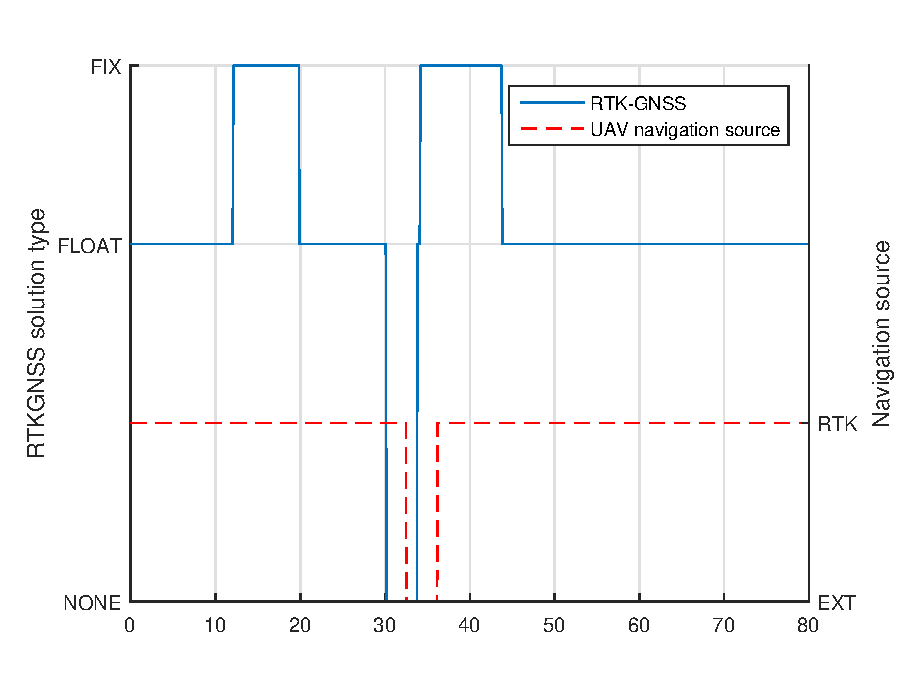
\includegraphics[scale=0.7]{figs/Experiment/navSource.eps}
\caption{State of \gls{rtk-gnss} system and \gls{uav} navigation source.}
\label{Fig:NavSource}
\end{figure}
\begin{figure}[H]
\centering
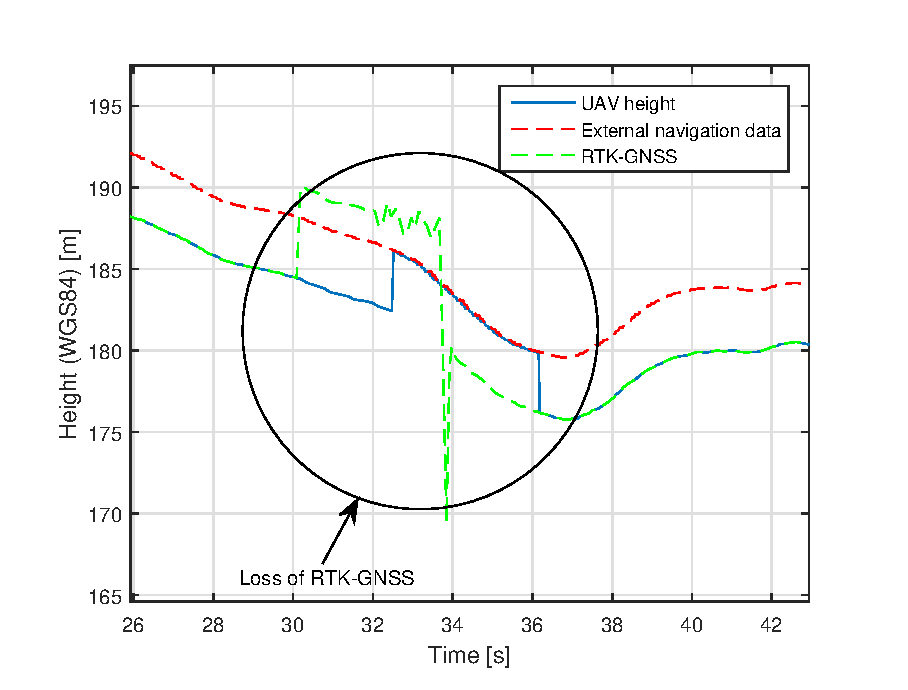
\includegraphics[scale=0.7]{figs/Experiment/shortrtkloss1juni114124.eps}
\caption{Loss of \gls{rtk-gnss} triggers the short loss compensator such that the \gls{uav} keeps the \gls{rtk-gnss} position solution longer}
\label{Fig:ShortLoss}
\end{figure}
\begin{figure}[H]
\centering
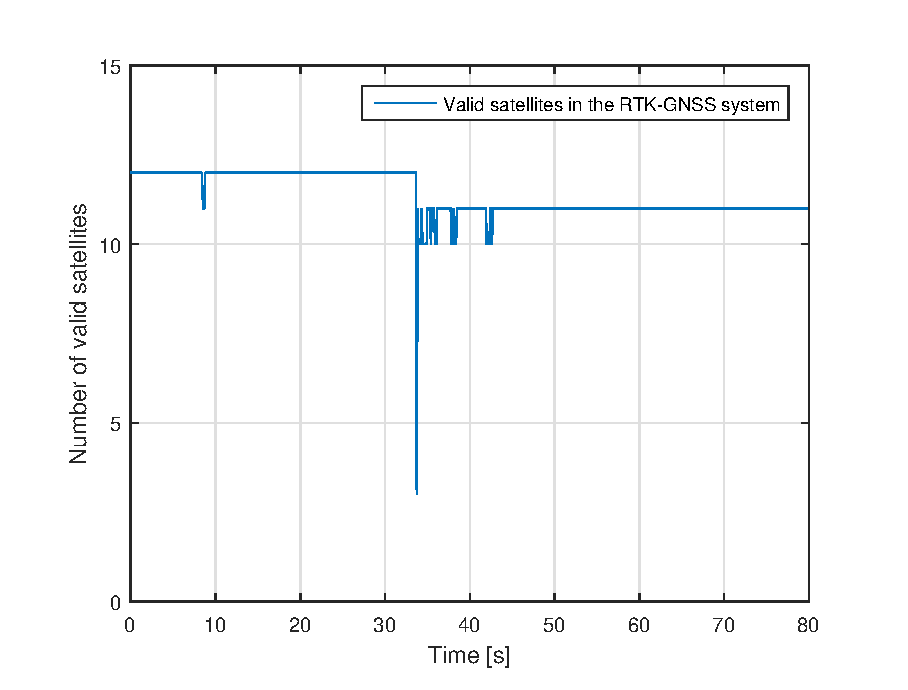
\includegraphics[scale=0.7]{figs/Experiment/ShortrtklossSatellites1juni114124.eps}
\caption{Number of valid satellites during a flight mission}
\label{Fig:SatCount1juni114124}
\end{figure}
\subsection{Discussion}
The navigation system was able to provide high accuracy position solution to the \gls{uav} during the autonomous landing flight plan, however continues drop out of the \gls{rtk-gnss} system was experienced when the satellite geometry decreased, which make the positioning system more susceptible to atmospheric disturbance. The drop out may be reduced by increasing the elevation mask in RTKlib. In order for the system to be able to perform during a prolong duration of degraded satellite geometry a state estimator must be created which can give a accurate position estimate with minimum \gls{rtk-gnss} information available. This would be a more advance estimator compared to the short loss compensator presented in this thesis.

The short loss compensator was able to compensate the solution from the external navigation system sufficiently to avoid a large step in \gls{uav} position data for the short period where the \gls{rtk-gnss} data was not available. However the limits of the short loss compensator has yet to determined, and should be further tested. The goal of the navigation system is be to be able to provide high accurate position solution to the \gls{uav}, even if the \gls{rtk-gnss} system experience a drop out.
\section{Path system performance}
\subsection{Experimental results}
The construction of the approach path with respect to the wind direction resulted in a non optimal path for the \gls{uav} in the initial set-up and test set-up 2, section \ref{ss:TestSetup1} and section \ref{ss:Day1FinalApp} respectively. The combination of flying in the cross wind and a non smooth transition into the finish turning circle gave oscillation in the North-East plane. Inverting the start turning circle in test set-up 3, section \ref{ss:Day1Inverted}, resulted a smoother transition between the two turning circles and reduced oscillation in the North-East plane.

The landing path direction was chosen such that the \gls{uav} had to land in the head wind. This resulted in the \gls{uav} to have a lower ground speed then the measured air speed, as seen in figure \ref{Fig:Airspeed31mai125420} which is part of test set-up 3, section \ref{ss:Day1Inverted}. In the same figure, it is shown that the cross track error correlated to whether or not the \gls{uav} is flying in the head wind. The result of flying in the head wind is a lower cross track error compared to when in the tail wind.
\newpage 
\begin{figure}[H]
\centering
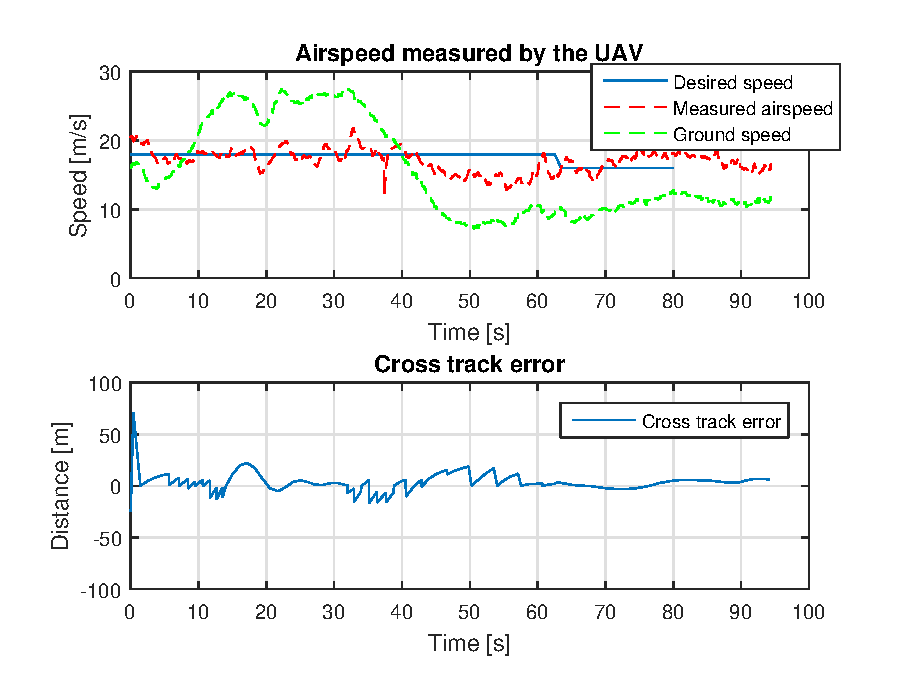
\includegraphics[scale=0.9]{figs/Experiment/airspeed31mai125420.eps}
\caption{Measured airspeed and ground speed together with desired airspeed. In addition, the cross track error for the same landing plan mission}
\label{Fig:Airspeed31mai125420}
\end{figure}

Reducing the arc segment distance of the turning circles in the approach path in test set-up 6, section \ref{ss:Day2ArcDistance}, resulted in a smoother circle which  was more suitable for the \gls{uav} to follow. The effect of reduced arc segment distance for the lateral control system performance is discussed further in section \ref{ss:EvaluationControl}.

The final approach angle was identified to cause a problem where the desired height didn't converge to the net center heigh at the time where the \gls{uav} passed the net. The reason for this behaviour is explained further in section \ref{ss:EvaluationControl}. In test set-up 2, section \ref{ss:Day1FinalApp}, the final approach angle was set to $0 \deg$, resulting in a straight line through the net with a constant height.

Test set-up 5, section \ref{ss:Day2GlideSlope} showed that a glide slop angle greater then $6 \deg$ resulted in the autonomous landing system being unable to follow the desired height during the final phase of the landing plan. The reason for why the control system is unable to follow a steeper decent angle then $6 \deg$ is discussed further in section \ref{ss:EvaluationControl}. An stationary net landing at from the East at Agdenes with the autonomous landing system will require a start altitude of the landing path at $56 m$ above the runway. At this altitude the \gls{uav} will have a safe distance from the highest tree tops when in the final turning circle. With a glide slope angle of $6 \deg$ and final approach angle of $0 \deg$ the necessary length of the glide slope would be $500 m$.
\subsection{Affecting parameters}
The rotation combination for the turning circles in the approach path was identified to result in increased performance for the lateral control system, given that they had the same rotation direction. Thus the combination of rotation direction should be considered carefully, with the recommended combination being either counter-clockwise/counter-clockwise or clockwise/clockwise. Combined with an reduced arc segment distance in the turning circles, which resulted in the lateral control system holding a high desired roll angle, the oscillation and overshot was almost removed.

Attempts to increase the start height of the landing path allowed for the identification of the maximum glide slope angle which the longitudinal control system can follow in the X8 fixed-wing \gls{uav} hardware configuration. In addition, the final approach angle was required to be $0 \deg$, in order for the straight line which runs through the net center has a constant height. This is necessary if the desired height from longitudinal control system should converge to the net center height.

Key landing plan parameter with recommended values for increase autonomous landing system performance are listed in table \ref{Tb:RecommmendedLandingPlanParameter}.
\begin{table}[H]
\centering
\begin{tabular}{| l | l |}
\hline
\textbf{Parameter name}			&  \textbf{Recommended value} 	\\ \hline
Time of arrival factor			&	$2 s$						\\ \hline
Distance between arc segments	&	$10 m$					 	\\ \hline
Final approach length			&	$100 m$					 	\\ \hline
Final approach angle			&   $0 \deg$					\\ \hline
Glide slope angle				&	$6 \deg$				 	\\ \hline
\end{tabular}
\caption{Recommended parameter alteration to the landing plan with respect to the plan parameter given in table \ref{AP:TB:landingDay2}, and the task configuration parameter given in table \ref{Tb:LandingPlanParameter}}
\label{Tb:RecommmendedLandingPlanParameter}
\end{table}
\subsection{Discussion}
The minimum height from which the autonomous landing system could start the landing path from was found to be $56 m$ above the runway at Agdenes airfield when attempting to land from the East. This strain the operation boundaries in which the \gls{uav} operates, since the approach could move the \gls{uav} out of the line of sight of the pilot. An alternative approach from the west is possible, however the typical wind condition on Agdenes is from the west. Thus landing from the west can only be performed during calm wind conditions. Other path alternative has yet to be attempted, however environmental obstacles around the runway limit the viable path options.

Attempts to increase the glide slope angle resulted in the \gls{uav} passing the net with a height error larger enough to miss the net. Further attempt should be made with a better tuned system. However, the risk with an increased glide slope angle is an increased airspeed, which could result in a large overshot with respect to the desired height.
\section{Control system performance}\label{ss:EvaluationControl}
\subsection{Experimental results}
\subsubsection{Longitudinal control system}
The experimental testing in test set-up 1 in section \ref{ss:TestSetup1} showed that the longitudinal control system was unable to converge to the net center height due to the reference model used to smooth up the desired height. The longitudinal control system require a constant path height in order for the desired height to converge to the path, which was shown in test set-up 2 in section \ref{ss:Day1FinalApp}.

Attempts to increase the glide slope angle of the landing path greater then $6 \deg$ resulted in the longitudinal control system being unable to pass the net within the acceptance criteria for net passing, given in table \ref{tb:NetCriteria}. A key reason for this behaviour is the inability of the \gls{uav}s low level pitch controller to follow the desired pitch, as shown in figure \ref{Fig:Pitch1juni081328} from test set-up 5 in section \ref{ss:Day2GlideSlope}.
\newpage
\begin{figure}[H]
\centering
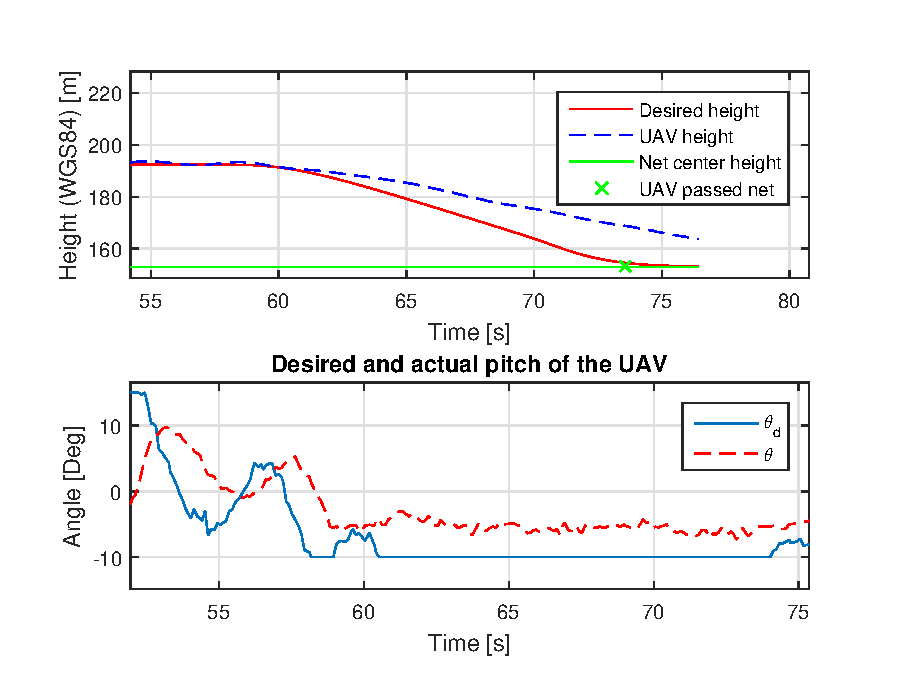
\includegraphics[scale=0.7]{figs/Experiment/Pitch1juni081328.eps}
\caption{Desired $\theta_d$ and actual pitch $\theta$, of the \gls{uav} at the time the \gls{uav} is in the glide slope}
\label{Fig:Pitch1juni081328}
\end{figure}
The overall net passing performance of the longitudinal control system shows that the \gls{uav} mostly passed over or in the upper part of the net. This is a result of the high average error in the overall performance identified in table \ref{tb:Day1HeightCrossTrack} and \ref{Tb:AverageCrossHeightDay2}.

\subsubsection{Lateral control system}
The oscillation motion in the North-East plane was significant during both days of testing, resulting in a high variance of the average error in table \ref{tb:Day1HeightCrossTrack} and \ref{Tb:AverageCrossHeightDay2}. The lateral oscillation motion affect the net passing results, where the cross track error is spread evenly along the cross track axis in figure \ref{Fig:Day1NetPass}. However the cross track error for the net passing during the second test day gave a centred result, where the cross track error from all flight was grouped around the center of the cross track axis, as seen in figure \ref{Fig:Day2NetPass}. Reduction of the lookahead distance in the lateral control system in test set-up 4, section \ref{ss:Day1:ReducedLookahead}, resulted in reduction of oscillation motion in the north-east plane.

The \gls{uav} experienced overshot when attempting to follow the path in one of the turning circles. By reviewing the desired roll ($\phi_d$ ) and the actual roll ($\phi$) of the \gls{uav} at the time of the final turn, shown in figure \ref{Fig:DesiredRoll131844} from test set-up 4 in section \ref{ss:Day1:ReducedLookahead}, it's observed that the lateral control system decrease the desired roll in the middle of the turn.
\begin{figure}[H]
\centering
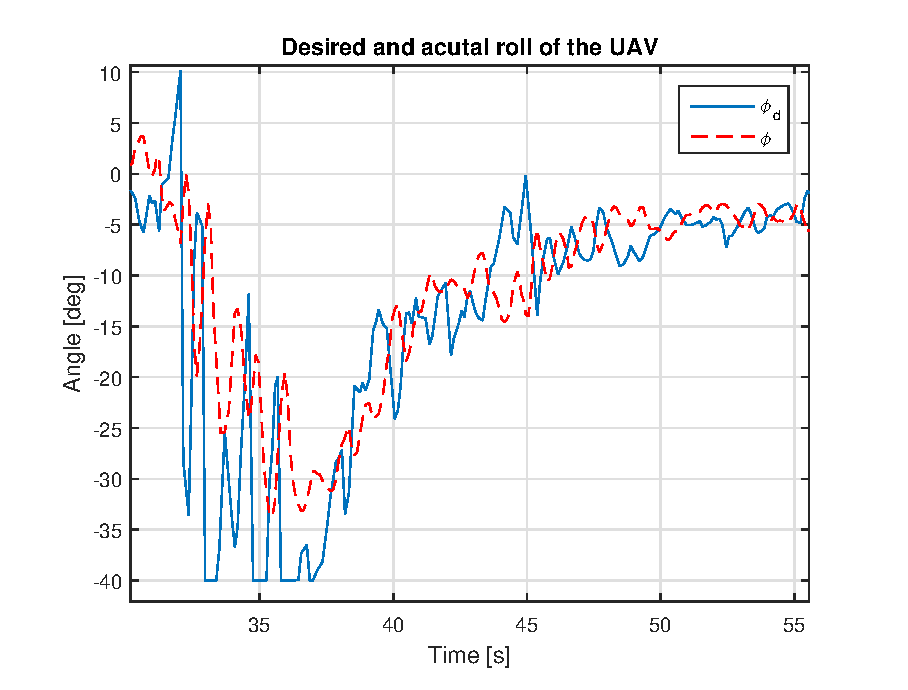
\includegraphics[scale=0.7]{figs/Experiment/rollDesired131844.eps}
\caption{The desired roll and actual roll of the \gls{uav} during the finish turning circle}
\label{Fig:DesiredRoll131844}
\end{figure}
The overshot in the start circle is a result of the roll angle not being able to follow the desired roll angle fast enough, as seen in figure \ref{Fig:Roll1juni081328} from test set-up 5 in section \ref{ss:Day2GlideSlope}.
\newpage
\begin{figure}[H]
\centering
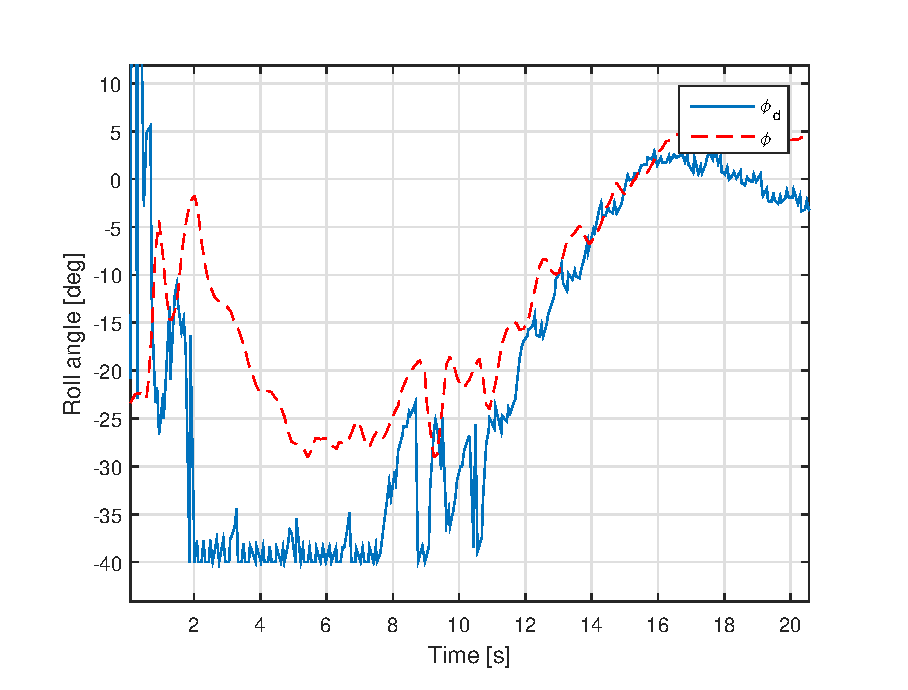
\includegraphics[scale=0.7]{figs/Experiment/Roll1juni081328.eps}
\caption{Desired and actual roll angle during the start turning circle}
\label{Fig:Roll1juni081328}
\end{figure}
The overshot in the finish turning circle was reduced after adjustment where made to the arc segment distance in the turning circles. The desired behaviour where the lateral control system keep a high desired roll angle through is achieved and shown in figure \ref{Fig:RollFinalTurning083423} from test set-up 6 in section \ref{ss:Day2ArcDistance}.
\newpage
\begin{figure}[H]
\centering
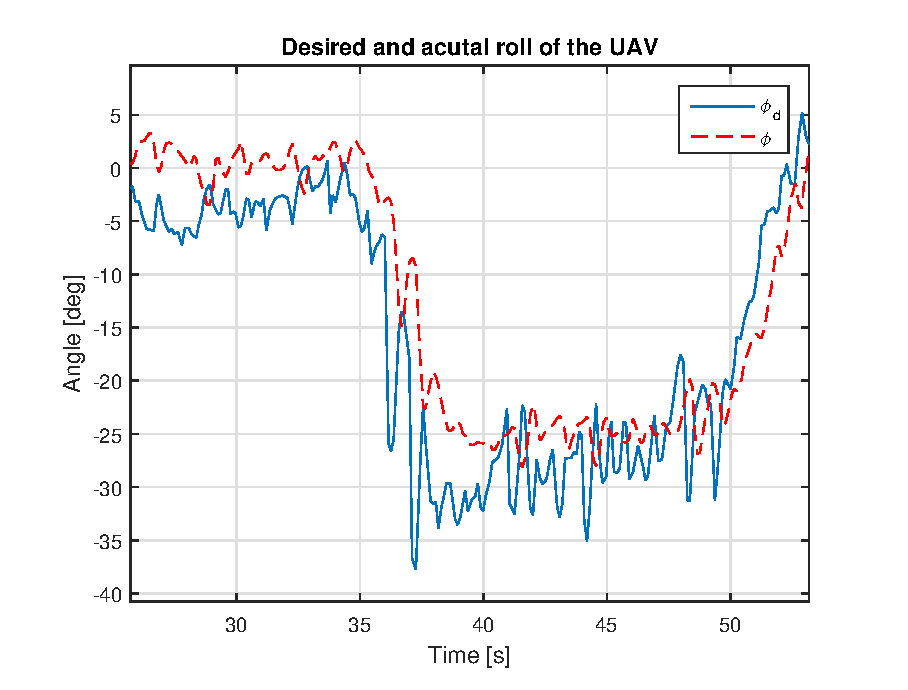
\includegraphics[scale=0.7]{figs/Experiment/Roll1juni083423.eps}
\caption{Roll and desired roll in the final turning circle}
\label{Fig:RollFinalTurning083423}
\end{figure}
\subsection{Affecting parameters}
Reduction of the lookahead distance in the lateral control system resulted in a more aggressive controller towards wind disturbance, increasing the performance when flying in the head wind. This is not beneficial when flying in the tail wind since the \gls{uav} will then lack control surface to compensate for the wind disturbance.
\subsection{Discussion}
The longitudinal control system showed a stable performance, but a large average error in the height with respect to the desired height showed a performance that is not acceptable for an autonomous landing system. The results obtain in the \gls{sil} simulation in section \ref{SIL:Results}, where the low level controllers are fined tuned, shows that the performance can be increased by further tuning of the low level pitch controller.

The lateral control system performed with satisfying result during the second day when the wind condition was calm, but during the first day it experienced problems when attempting to converge to the straight line between two waypoints. This result differ from the \gls{sil} simulation of the autonomous landing system, expected as the mathematical model used to represent the X8 \gls{uav} has not been verified against a physical model of the X8. In addition, the low level controllers has not been fined tuned for autonomous flights. The lateral control system  struggled to avoid overshooting when following the finish turning circle, with some resulting overshot large enough to bring the \gls{uav} to the edged of the operational flight space.

The lateral control system experience overshot during the turning manoeuvres in the approach path due to only seeing the next waypoint and not the turning circles as a whole. The lateral control system should be improved to use more information about the landing plan, when the desired path is smooth enough to follow.

The reduction of the lookahead distance will result in an increased performance when flying in the head wind, at the cost of reduced performance when flying in the tail wind. A possible solution to this problem would be to implement the lookahead distance as a function of the cross track error, which in \citep{fossen2011handbook} section 10.3.2 is given as:
\begin{equation}
\Delta(t) = \sqrt{R^2 - e(t)^2}
\end{equation}
where $\Delta(t)$ is the lookahead distance, $R$ is the maximum lookahead distance and $e(t)$ is the cross track error. In addition the lateral control system functionality could be expanded to increase the performance during a turning manoeuvre, with the goal of reducing the overshot.
\section{Summary}
Experimental testing of the autonomous landing systems ability to land in a virtual net placed $26 m $ above the runway have been completed over the course of two days with significant different weather conditions. The \gls{uav} used in the experiments was a X8 fixed wing \gls{uav}, described in section \ref{ss:X8andNest}. The different weather condition allowed for identification of strength and weaknesses with the control system, in addition to how alteration of landing plan parameters could affect the performance of the control system.

The path and control system in the autonomous landing system was able to create and follow a landing plan, resulting in mixed results. Strength and weaknesses with the proposed system was identified together with recommended landing plan parameters which can be used to ensure good performance from the autonomous landing system. The recommended landing plan parameters are listed in table \ref{Tb:RecommmendedLandingPlanParameter}. The performance of the lateral control system can be increase by making the lookahead distance a function of the cross track error. Further the low level controller for both roll and pitch must the fine tuned for autonomous flight, to increase the performance of both the lateral and longitudinal control system.

The navigation system performed with satisfying results, i.e. showed that it's able to provide a stable and reliable \gls{rtk-gnss} solution to the navigation system. The \gls{rtk-gnss} system is still prone to bad satellite geometry, which results in the \gls{rtk-gnss} system to loose satellite lock. During these events the short \gls{rtk-gnss} loss compensator is able to compensate the external navigation system, such that the navigation position solution remain at the same accuracy level as with \gls{rtk-gnss}. The time limitation in which the compensator is able to operate without divergence from the \gls{rtk-gnss} accuracy level is not concluded.